\documentclass[a4paper]{article}    % define document layout
%\documentclass[draft]{article}     % use draft option in packages
%-----------------------------
% preamble
%-----------------------------
\usepackage[sumlimits,]{amsmath}    % math equations and formulas
\usepackage[utf8]{inputenc}         % use UTF-8 encoding
\usepackage[english]{babel}         % use English language
\usepackage{graphicx}               % insert images
%\usepackage[draft]{graphicx}        % do not render figures
\usepackage{subcaption}             % multiple images in one figure
\usepackage{hyperref}               % hyperlinks
\usepackage{float}                  % floating objects (figures, tables)
\usepackage{geometry}               % page size and margins
\geometry{a4paper, margin=1in}      % margins
\usepackage{ragged2e}               % text alignment
\usepackage[table]{xcolor}          % change cell color in tables
%\usepackage{multirow}               % merge rows in table

\graphicspath{                      % path for figures
    {../figures/} 
    {../figures/alpha/} 
    {../figures/cm/} 
    {../figures/heatmap/} 
    {../figures/misclassified/} 
}

%-----------------------------
% body
%-----------------------------
\begin{document}

\begin{figure}
    \centering
    % UNICAMP logo
    \begin{subfigure}{0.45\textwidth}
        \centering
        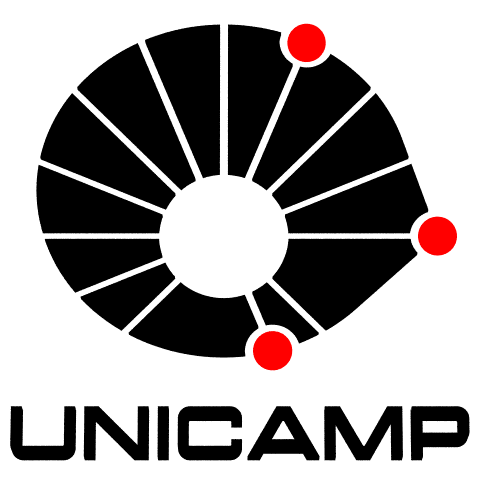
\includegraphics[width=1.5cm]{unicamp}
%        \label{fig:unicamp}
    \end{subfigure}
    \hfill
    % FEEC logo
    \begin{subfigure}{0.45\textwidth}
        \centering
        
\includegraphics[width=1.5cm]{feec}
%        \label{fig:feec}
    \end{subfigure}
\end{figure}

\title{
    \vspace{5cm}
    IA353A - Neural Networks\\
    EFC2 - Question 2
    \vspace{1cm}
}
\author{
    Rafael Claro Ito\\
    (R.A.: 118430)
    \vspace{11cm}
}
%R.A.: 118430
%ito.rafael@gmail.com
\date{May 2020}
\maketitle
\newpage

%=================================================
\section{Source files}
%=================================================

\paragraph{The Jupyter notebook with the code used to generate the plots and results presented in this report, all figures showed here and even the \LaTeX \space source code used to generate this PDF can be found at the following GitHub repository:}

\begin{center}
    {\url{https://github.com/ito-rafael/IA353A-NeuralNetworks-1s2020}}
\end{center}

%=================================================
\section{Extreme Learning Machine}
%=================================================

%-------------------------------------------------
\setcounter{subsection}{-1}
\subsection{Regularization coefficient (Ridge Regression)}
%-------------------------------------------------

\begin{table}[H]
    \begin{center}
        \begin{tabular}{r|c|c|} 
            \cline{2-3}
            & \multicolumn{2}{|c|}{\cellcolor[gray]{0.8}{$\lambda$ optimum}} \\
            \cline{2-3}
            & \cellcolor[gray]{0.8}{MSE} & \cellcolor[gray]{0.8}{Accuracy} \\
            \cline{1-3}
            \multicolumn{1}{|r|}{\cellcolor[gray]{0.8}{coarse search}} & 64   & 256   \\
            \cline{1-3}
            \multicolumn{1}{|r|}{\cellcolor[gray]{0.8}{fine search}}   & 102.7 & 662.7 \\
            \cline{1-3}
        \end{tabular}
    \end{center}
    \caption{Values of regularization coefficient found in coarse and fine searches}
    \label{tab:alpha_results}
\end{table}

%-------------------------------------------------
\subsubsection{Coarse search}
%-------------------------------------------------

\paragraph{While performing the coarse search for the best regularization coefficient, 3 more values of lambda were added. This was done in order to see the falling of the accuracy curve, even though the best accuracy was in $2^{8}$. The final values of lambda tested were:}

\begin{center}
    alpha\_interval = $[2^{-10}, 2^{-8}, 2^{-6}, 2^{-4}, 2^{-2}, 2^{0}, 2^{2}, 2^{4}, 2^{6}, 2^{8}, 2^{10}, \boldsymbol{2^{11}, 2^{12}, 2^{13}}]$
\end{center}

\begin{figure}[H]
    \centering
    % digit 0
    \begin{subfigure}{0.48\textwidth}
        \centering
        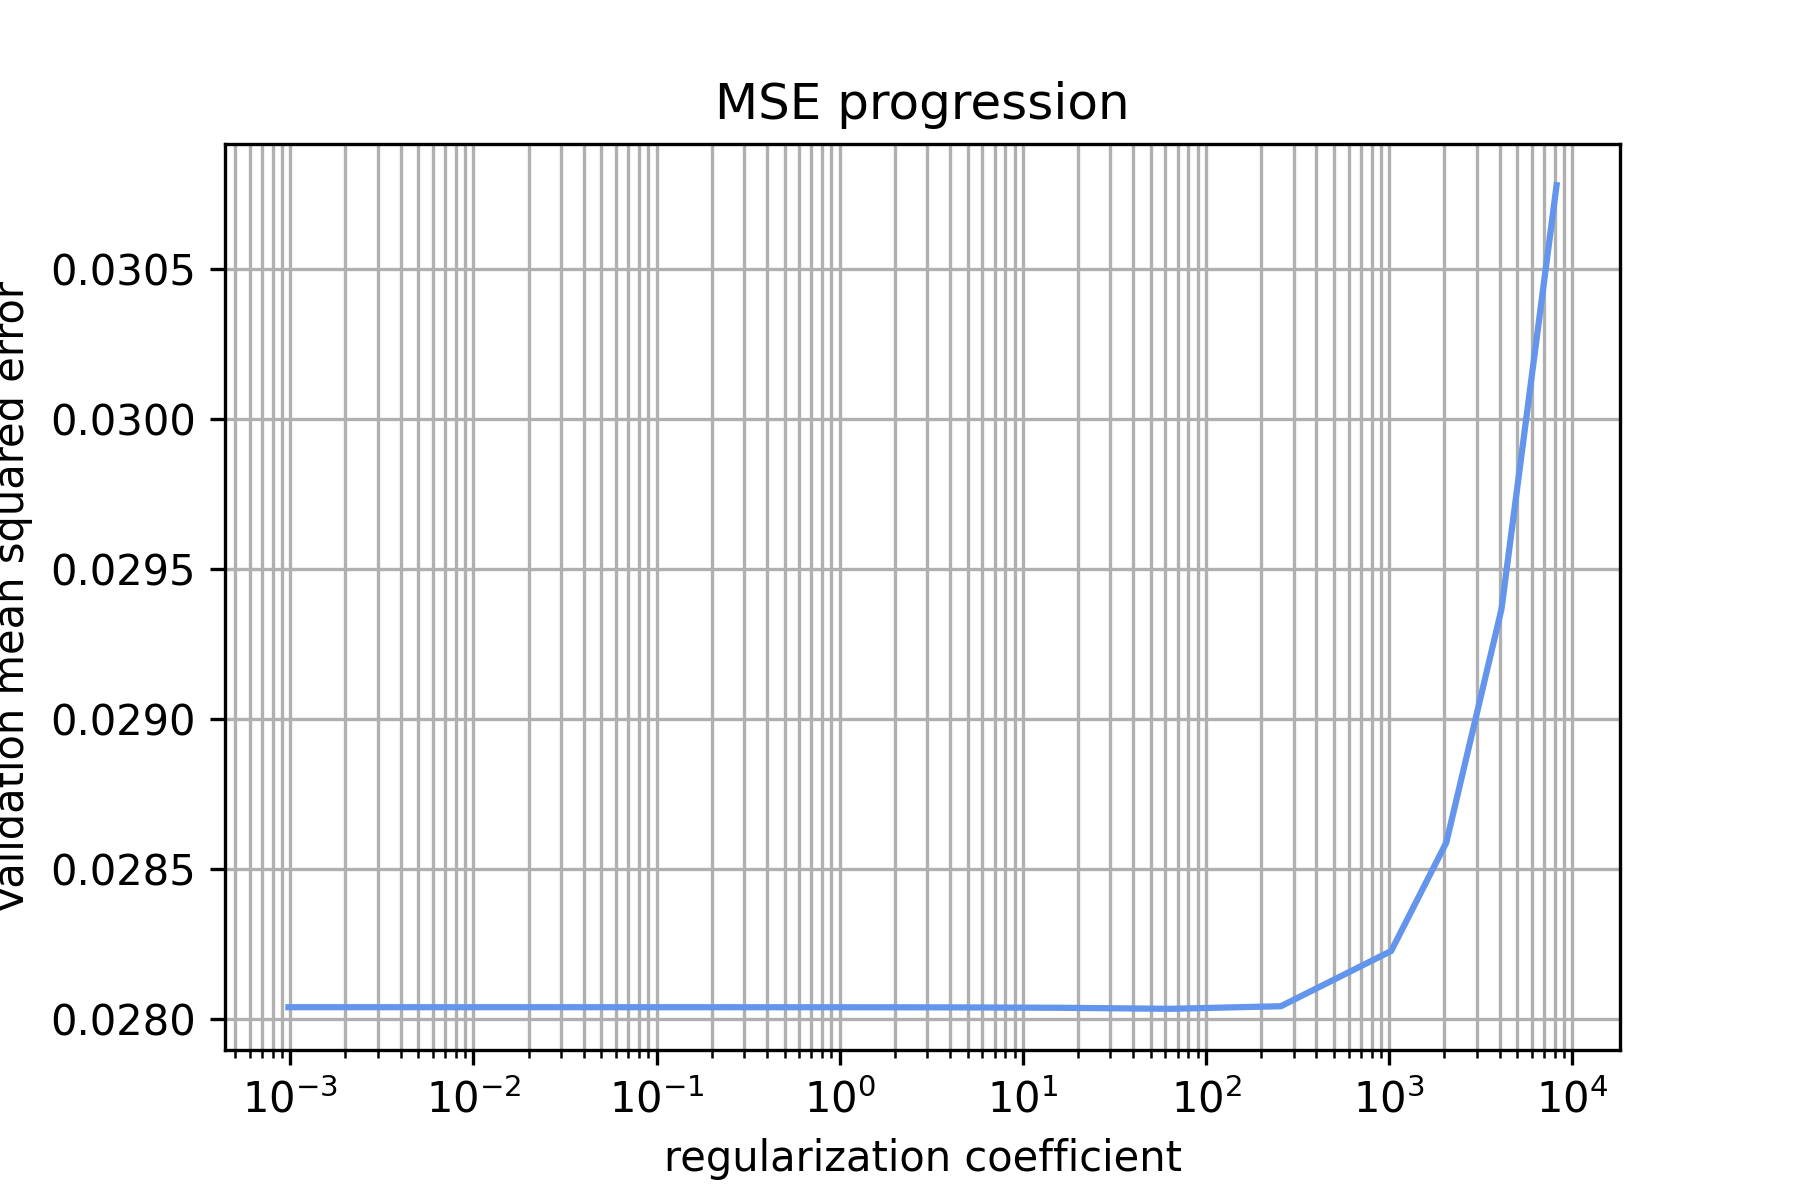
\includegraphics[width=7.5cm]{alpha_MSE_coarse_search}
        \caption{MSE progression}
        \label{fig:alpha-coarse-mse}
    \end{subfigure}
    \hfill
    % digit 1
    \begin{subfigure}{0.48\textwidth}
        \centering
        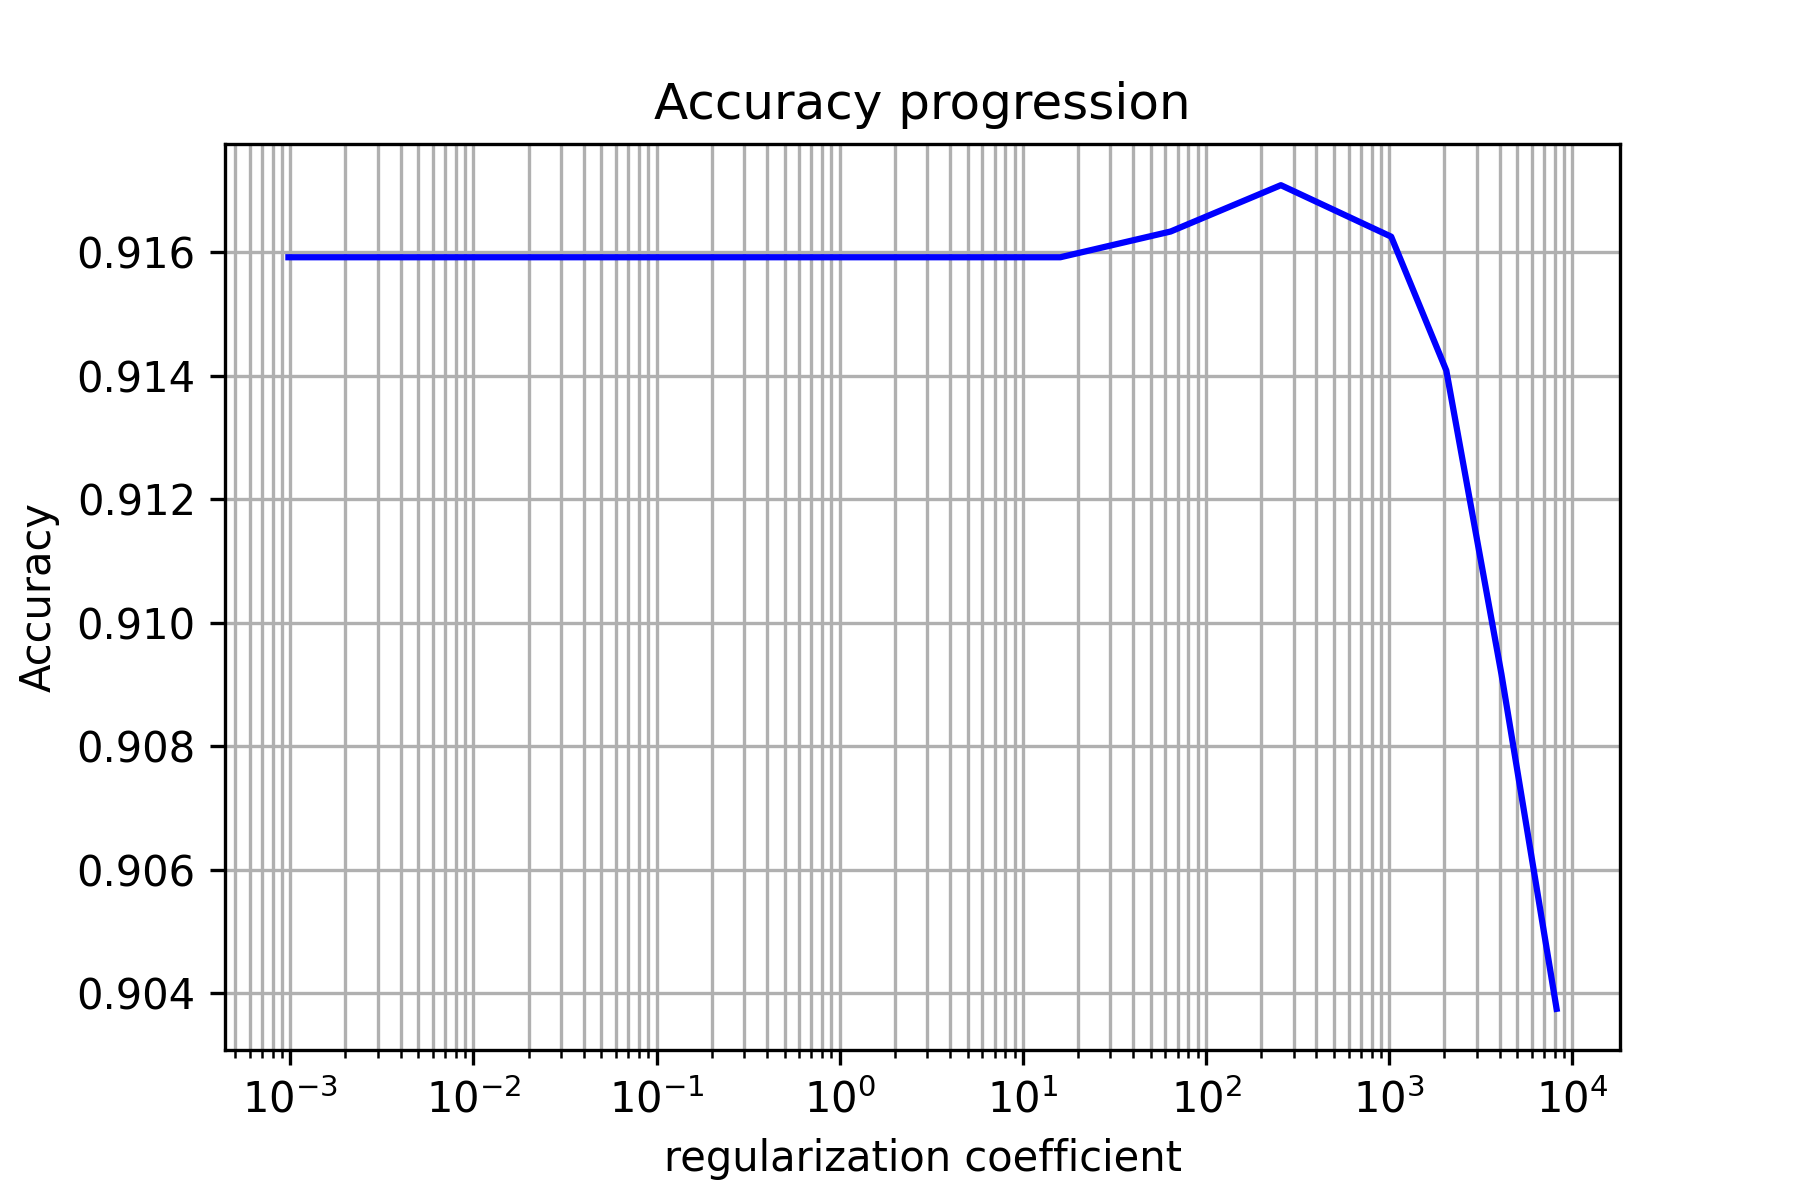
\includegraphics[width=7.5cm]{alpha_ACCURACY_coarse_search}
        \caption{Accuracy progression}
        \label{fig:alpha-coarse-acc}
    \end{subfigure}
    \hfill
    % caption and label
    \caption{Progression of MSE and accuracy in validation set for different values of the regularization coefficient (coarse search)}
    \label{fig:alpha_coarse}
\end{figure}

%-------------------------------------------------
\subsubsection{Fine search}
%-------------------------------------------------

\paragraph{In order to perform the fine search of the regularization coefficient, a golden-section one dimensional search algorithm was coded. Among the function parameters, the most important ones are the intervals of the search, precision desired and the loss function. The code can be found in:\\
\url{https://github.com/ito-rafael/machine-learning/blob/master/snippets/golden_section_search_valid.py}}

\begin{figure}[H]
    \centering
    % digit 0
    \begin{subfigure}{0.48\textwidth}
        \centering
        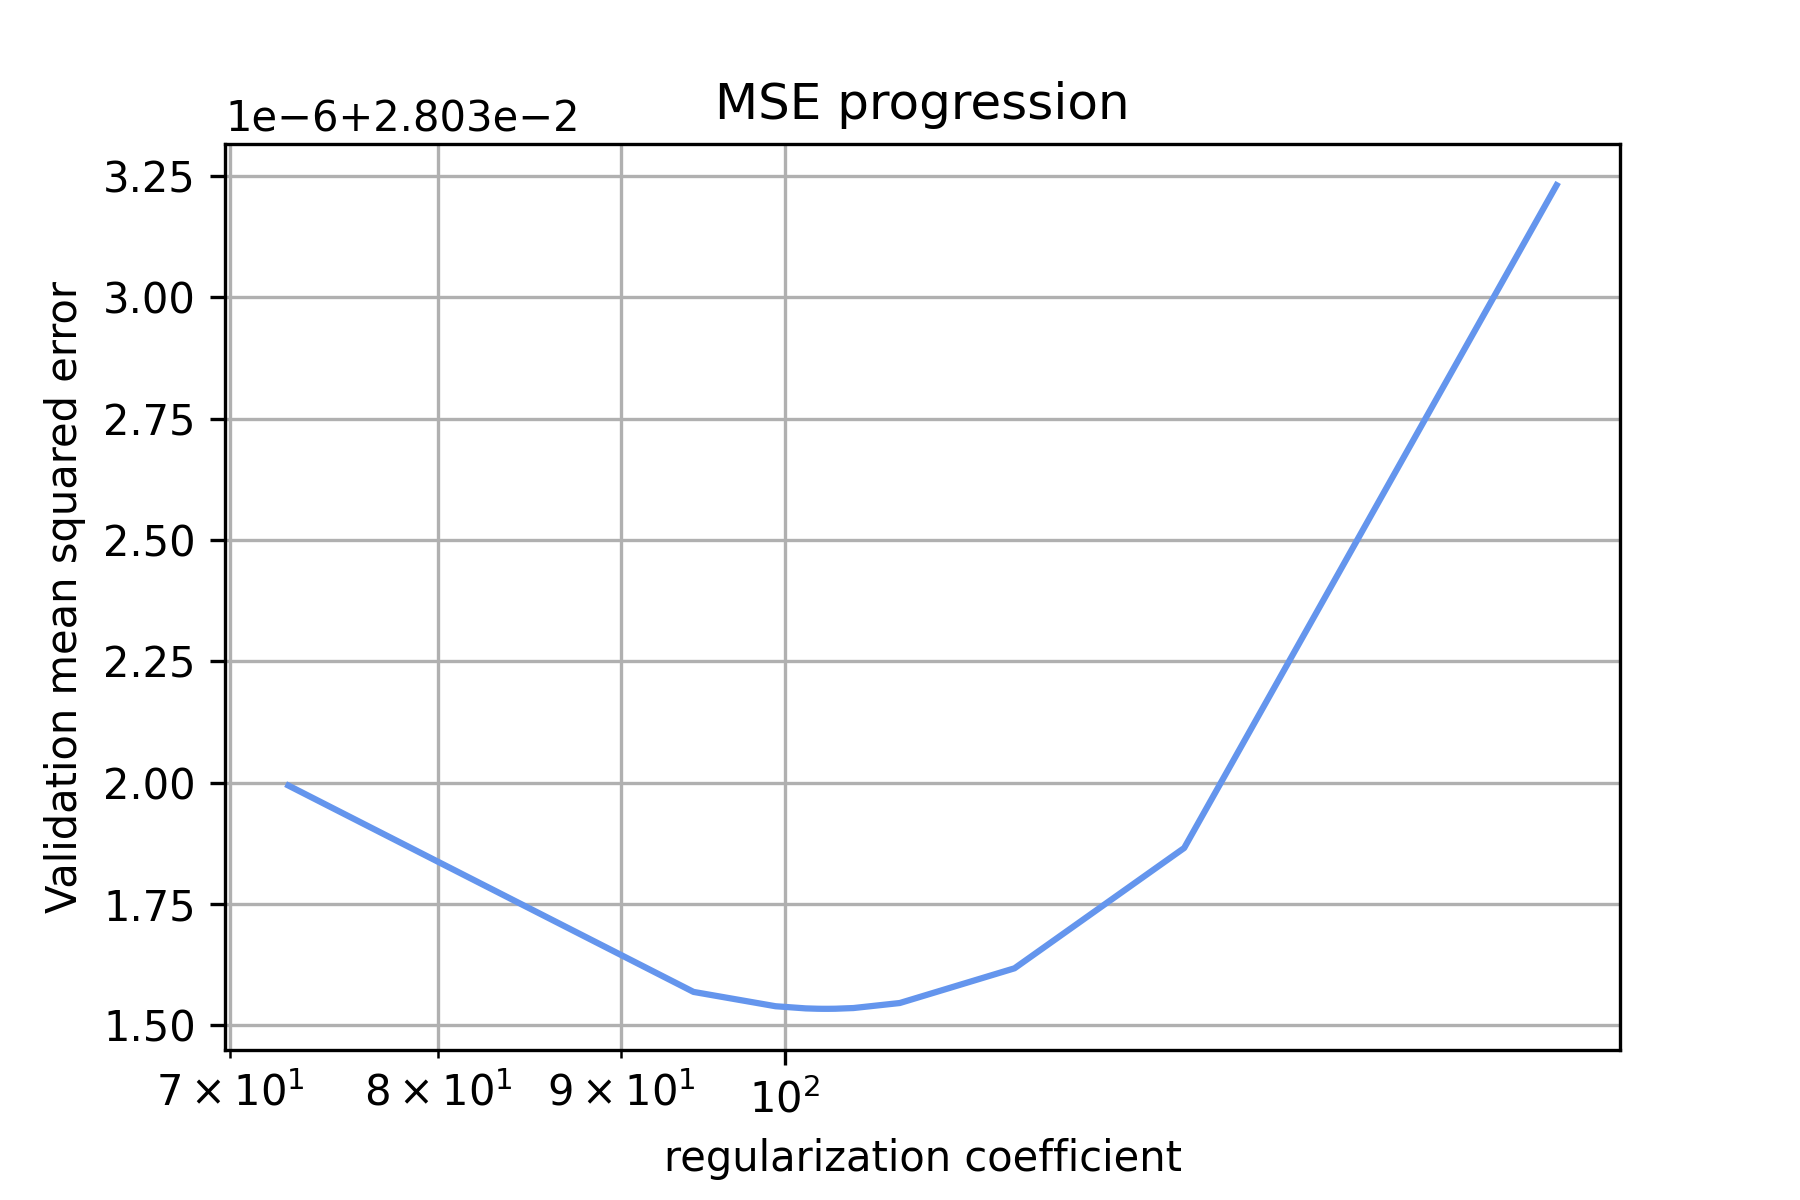
\includegraphics[width=7.5cm]{alpha_MSE_fine_search}
        \caption{MSE progression)}
        \label{fig:alpha-fine-mse}
    \end{subfigure}
    \hfill
    % digit 1
    \begin{subfigure}{0.48\textwidth}
        \centering
        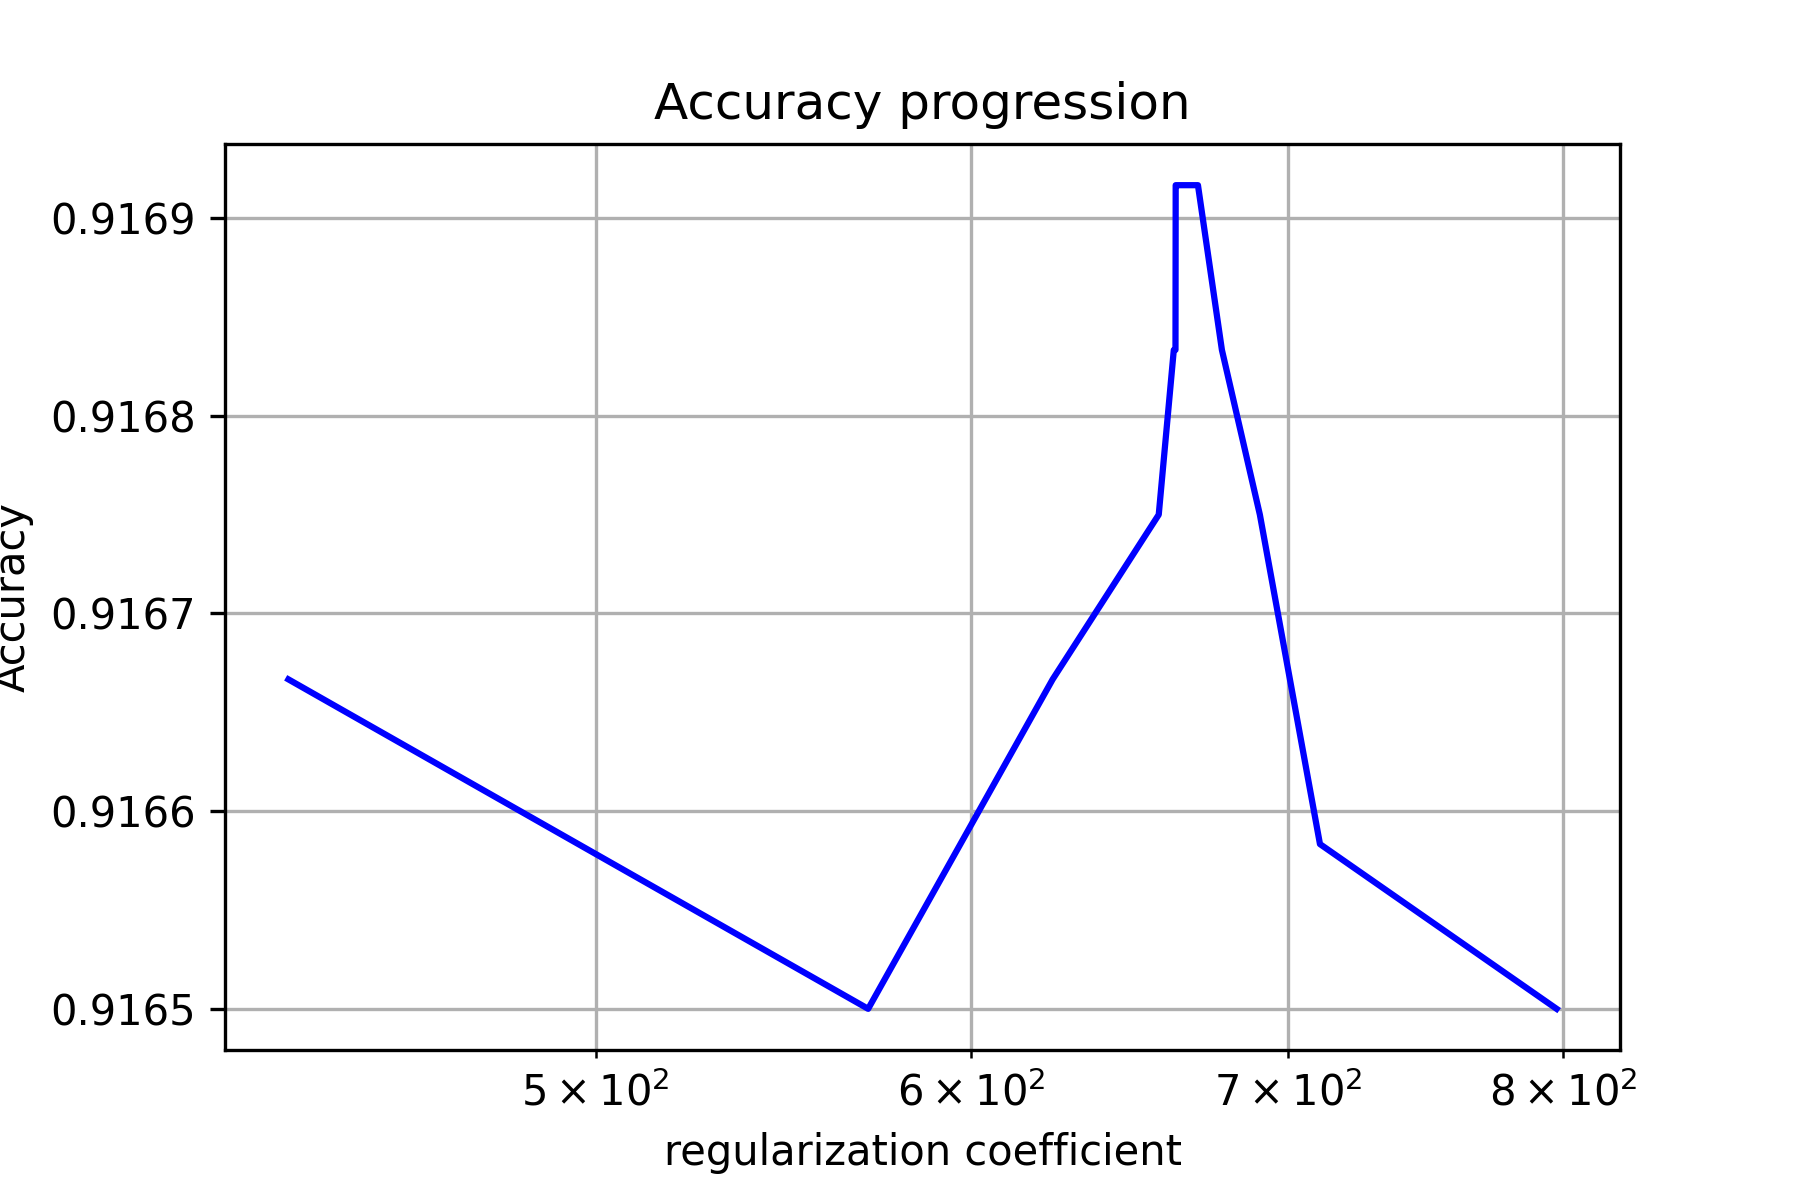
\includegraphics[width=7.5cm]{alpha_ACCURACY_fine_search}
        \caption{Accuracy progression)}
        \label{fig:alpha-fine-acc}
    \end{subfigure}
    \hfill
    % caption and label
    \caption{Progression of MSE and accuracy in validation set for different values of the regularization coefficient (fine search)}
    \label{fig:alpha_fine}
\end{figure}

%=================================================
\subsection{Confusion Matrix and Misclassification}
%=================================================

\paragraph{Considering the training set, plot the confusion matrix and a few examples of misclassified digits from at least three different classes.}

%-------------------------------------------------
\subsubsection{Confusion Matrix}
%-------------------------------------------------

\paragraph{The values displayed in the confusion matrix were obtained with the extreme learning machine applied to the training set (training plus validation). The training set is somewhat balanced, containing the number of samples for each class as illustrated in Figure \ref{tab:samples_training_set}}

\begin{table}[H]
    \begin{center}
        \begin{tabular}{|c|c|} 
            \cline{1-2}
            \cellcolor[gray]{0.8}{Digit} & \cellcolor[gray]{0.8}{nº of samples} \\
            \cline{1-2}
            0 & 5923 \\
            1 & 6742 \\
            2 & 5958 \\
            3 & 6131 \\
            4 & 5842 \\
            5 & 5421 \\
            6 & 5918 \\
            7 & 6265 \\
            8 & 5851 \\
            9 & 5949 \\
            \cline{1-2}
        \end{tabular}
    \end{center}
    \caption{Number of samples for each class in the training set}
    \label{tab:samples_training_set}
\end{table}

\begin{figure}[H]
    \centering
    % digit 0
    \begin{subfigure}{0.48\textwidth}
        \centering
        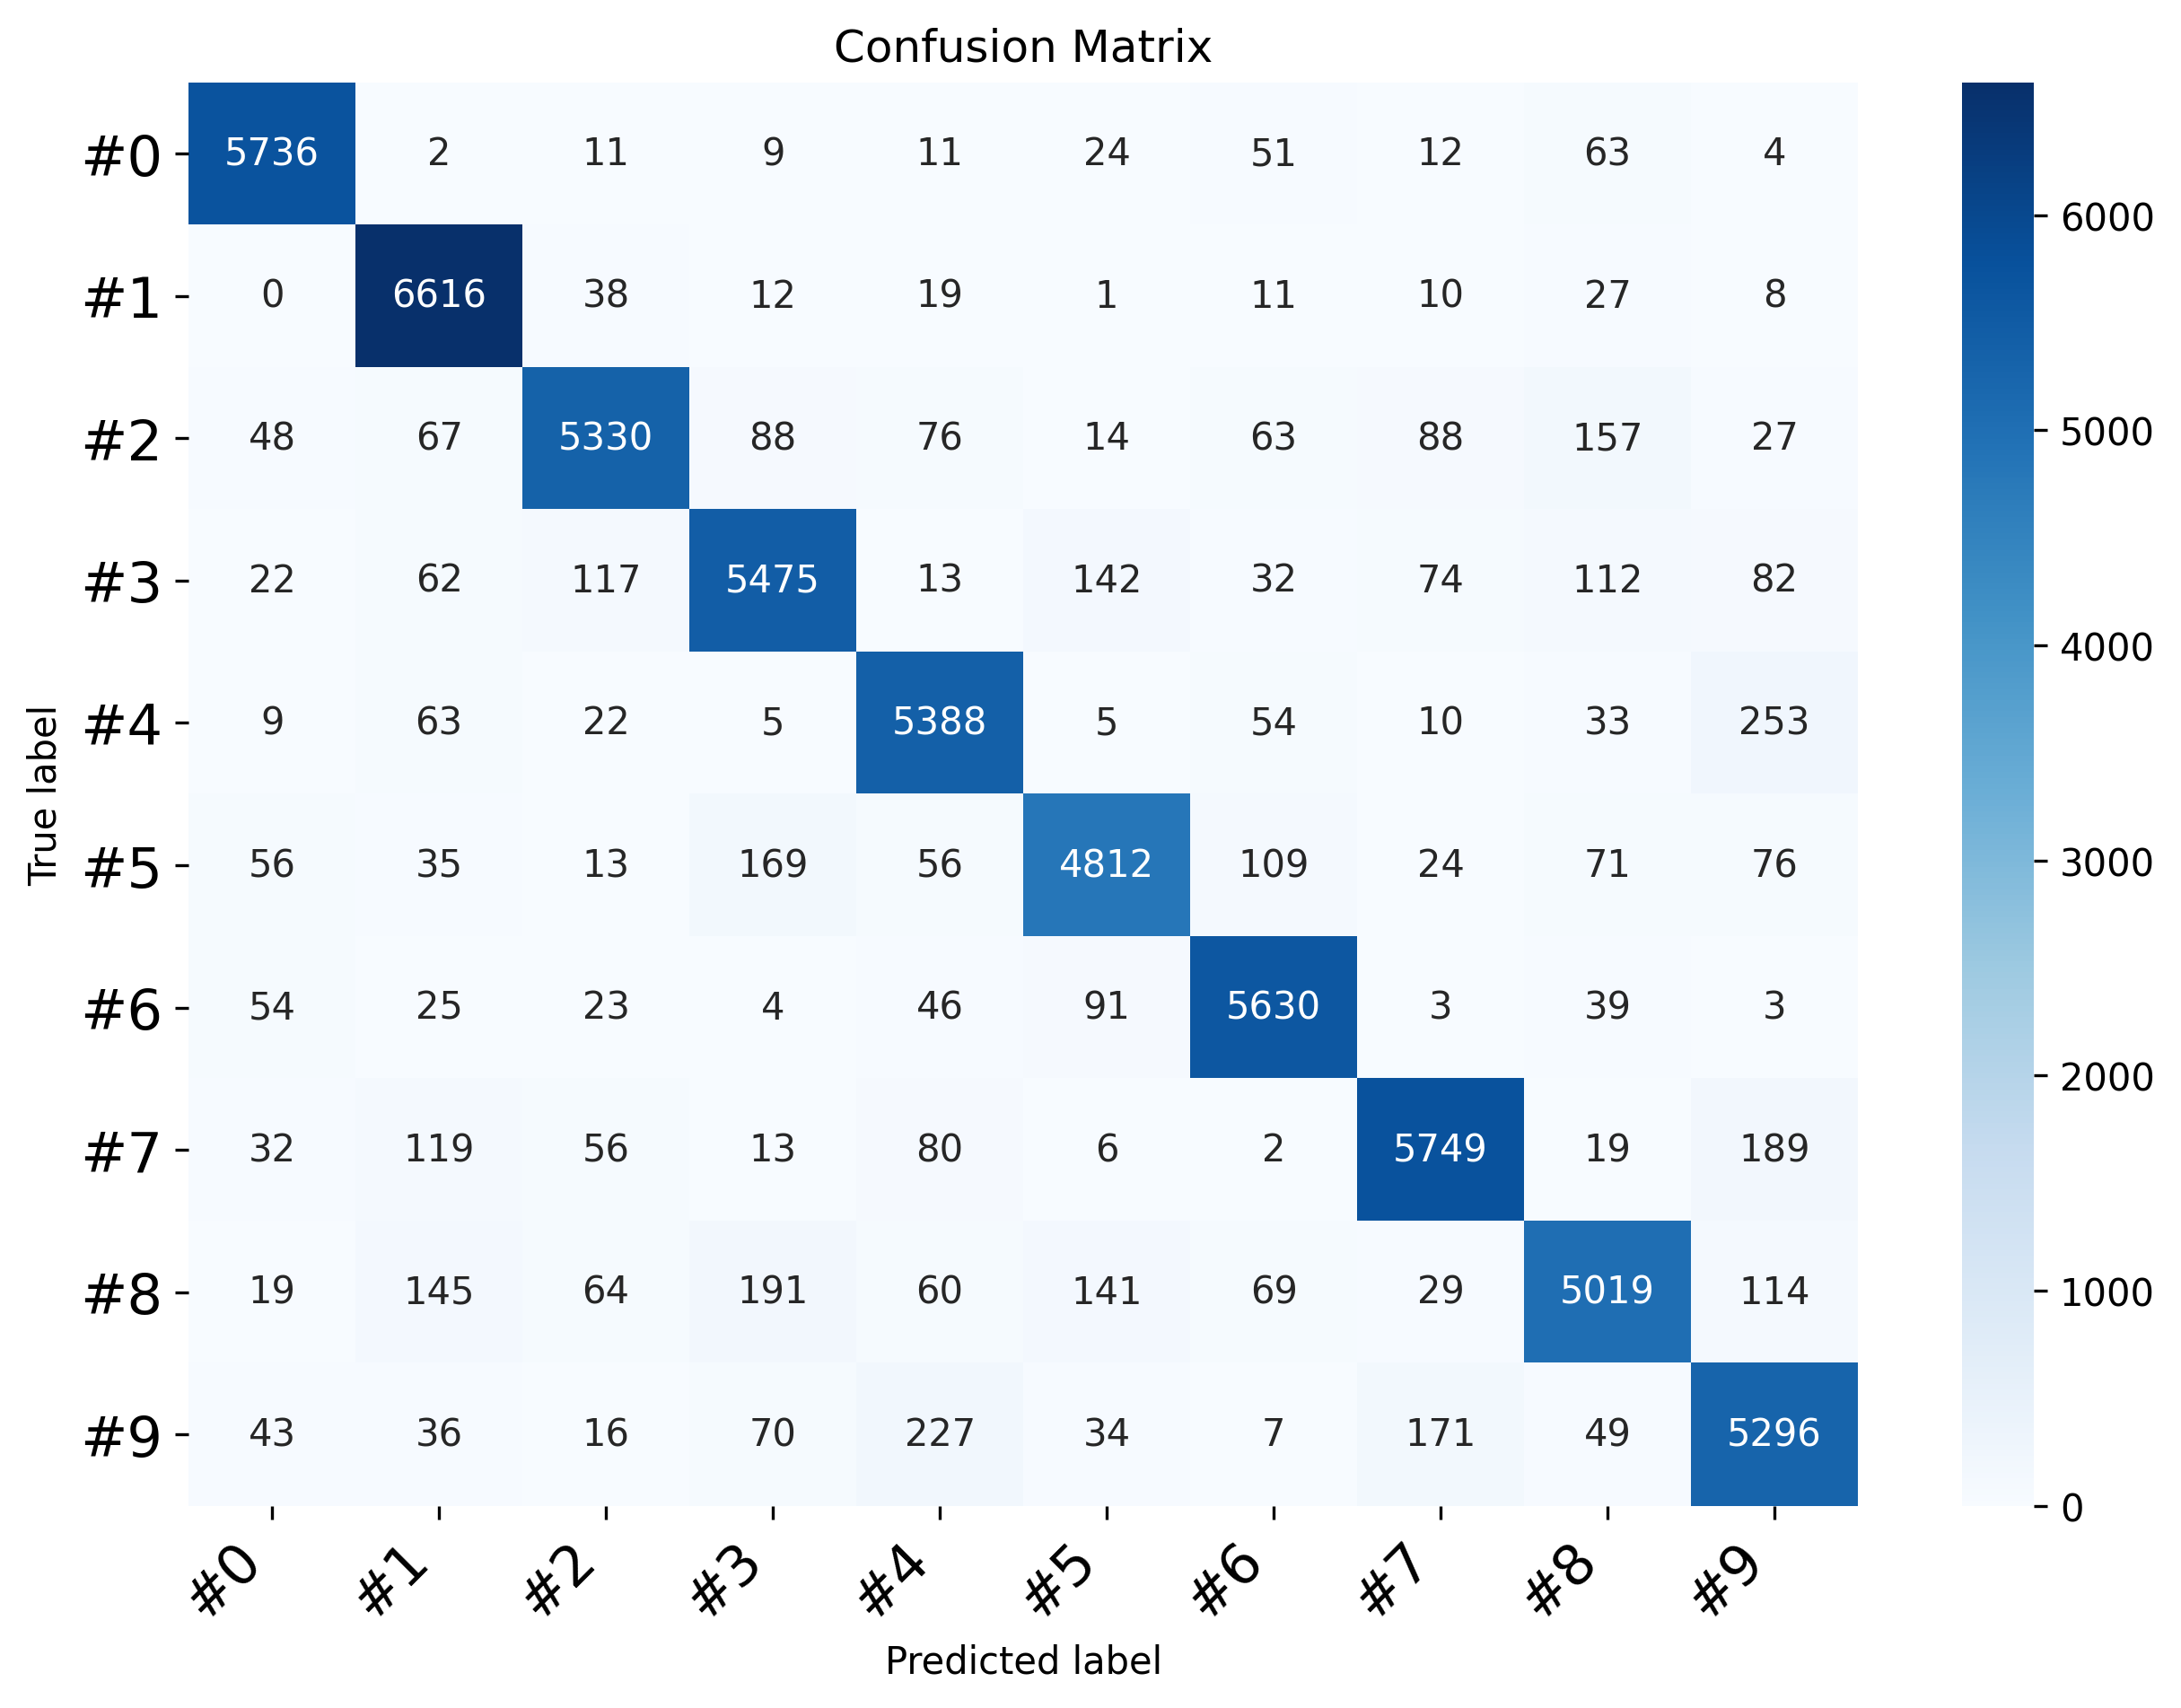
\includegraphics[width=7.5cm]{cm_raw}
        \caption{Confusion matrix with raw values}
        \label{fig:cm_raw}
    \end{subfigure}
    \hfill
    % digit 1
    \begin{subfigure}{0.48\textwidth}
        \centering
        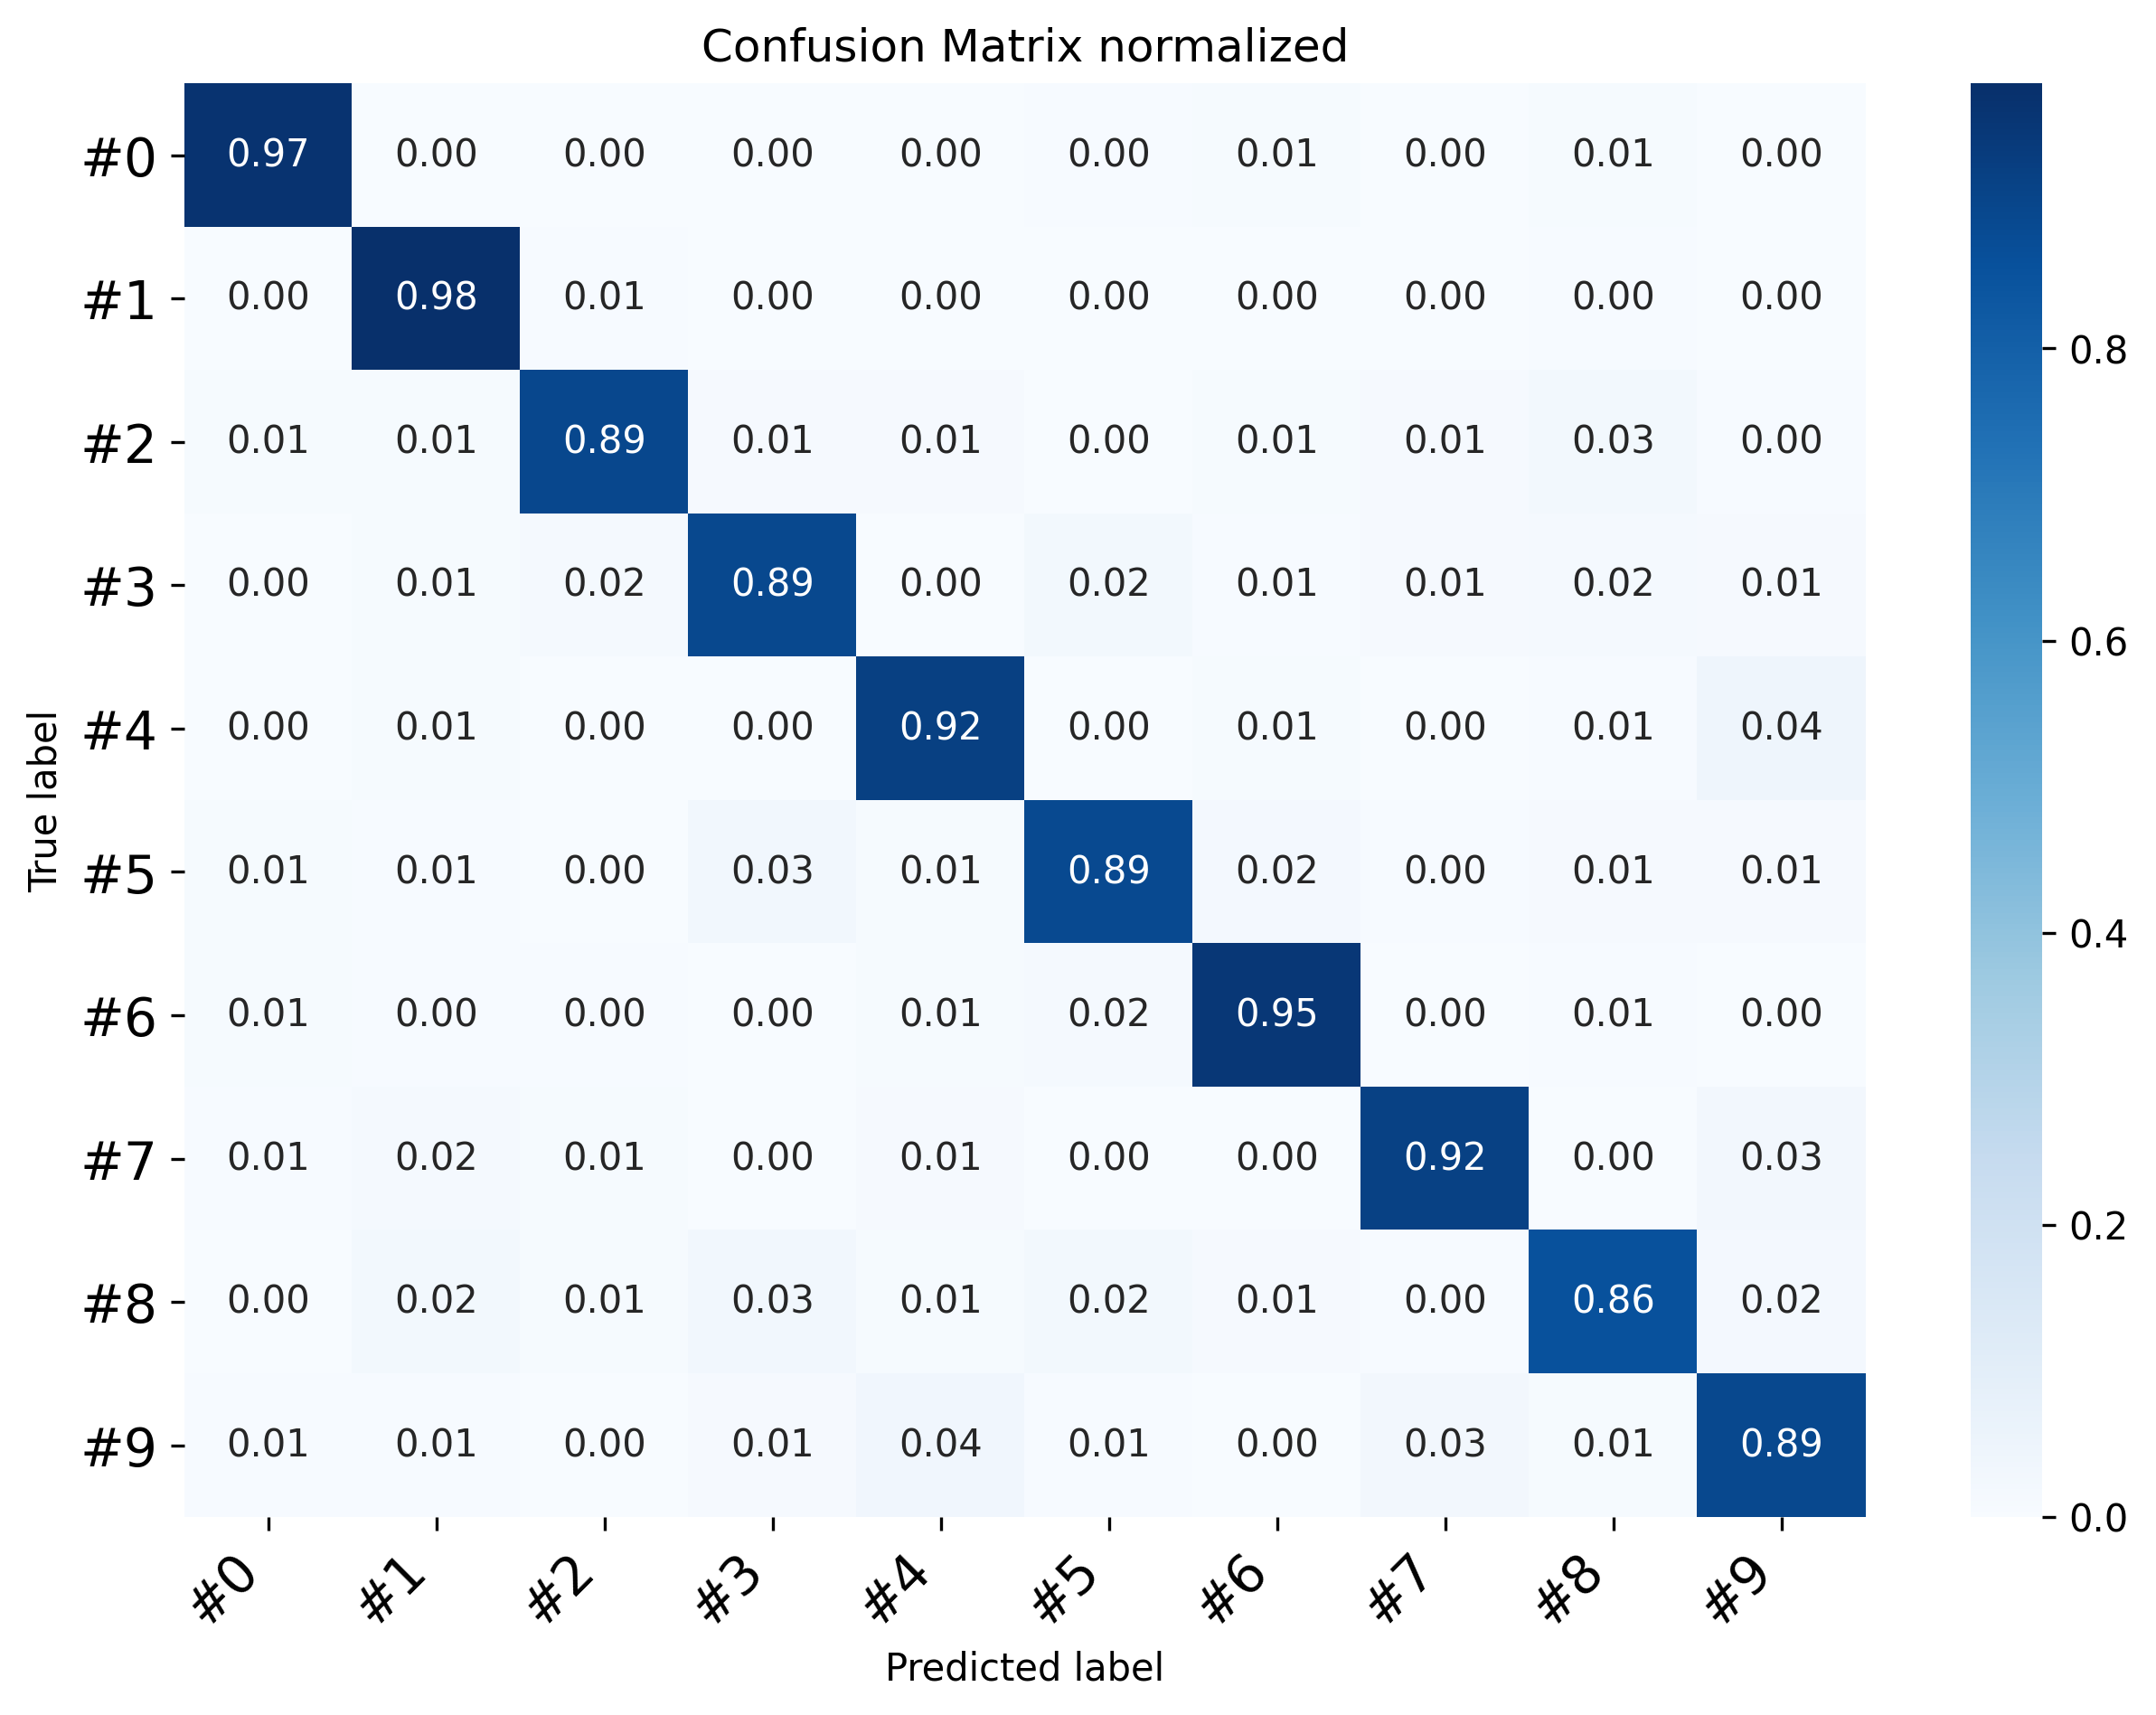
\includegraphics[width=7.5cm]{cm_norm}
        \caption{Confusion matrix with normalized values}
        \label{fig:cm_norm}
    \end{subfigure}
    \hfill
    % caption and label
    \caption{Confusion matrix with normalized and raw values} 
    \label{fig:cm}
\end{figure}

%-------------------------------------------------
\subsubsection{Misclassified data}
%-------------------------------------------------

\paragraph{The digits shown in Figure \ref{fig:misclassified_digits} are in the top 30 misclassified digits from which the difference between the output for the real class and the output for the predicted class are the highest. Both real and predicted class and its outputs values associated are indicated. The output is shown in parenthesis, in front of the correspondent class.}

\begin{figure}[H]
    \centering
    % example 1
    \begin{subfigure}{0.32\textwidth}
        \centering
        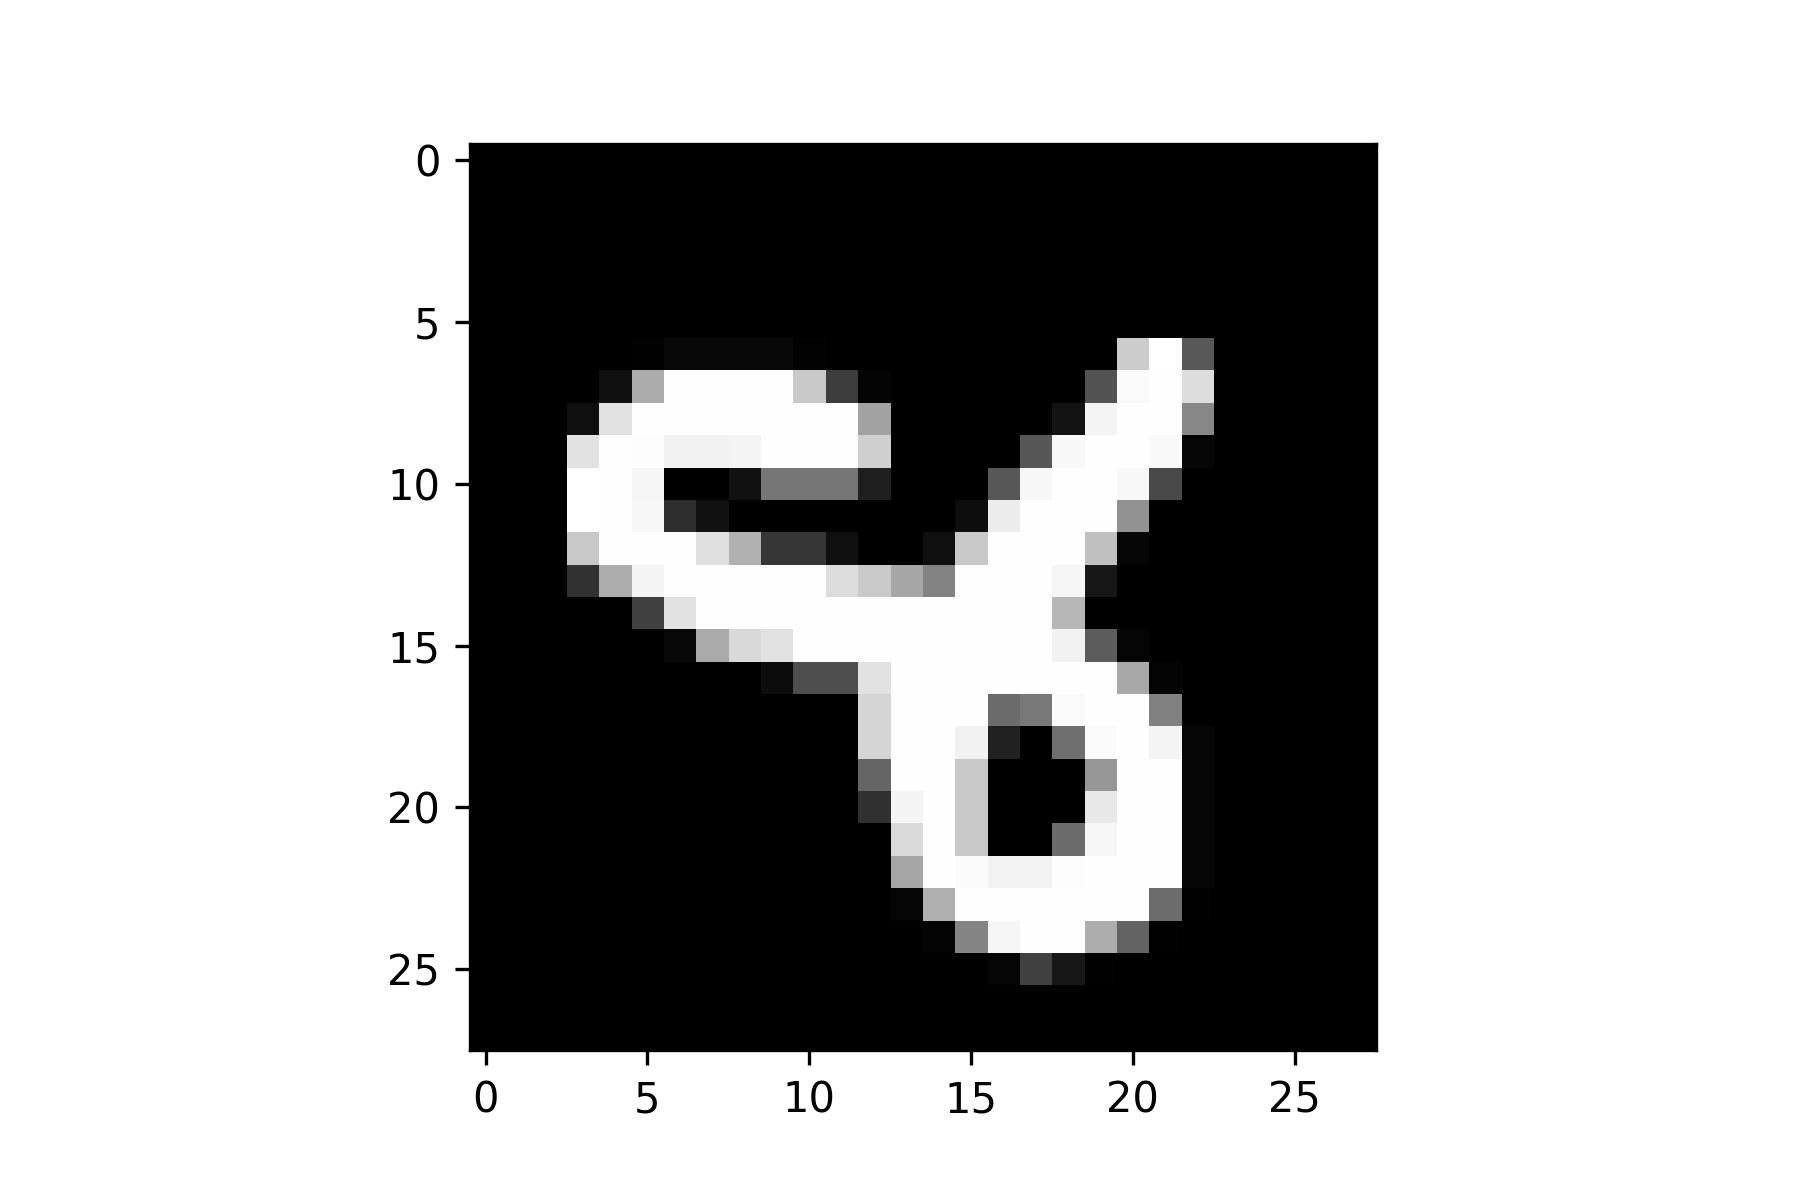
\includegraphics[width=5.0cm]{1}
        \caption{
            Real class: 3 (0.02)\\
            Predicted class: 7 (1.25)}
        \label{fig:example_1}
    \end{subfigure}
    \hfill
    % example 2
    \begin{subfigure}{0.32\textwidth}
        \centering
        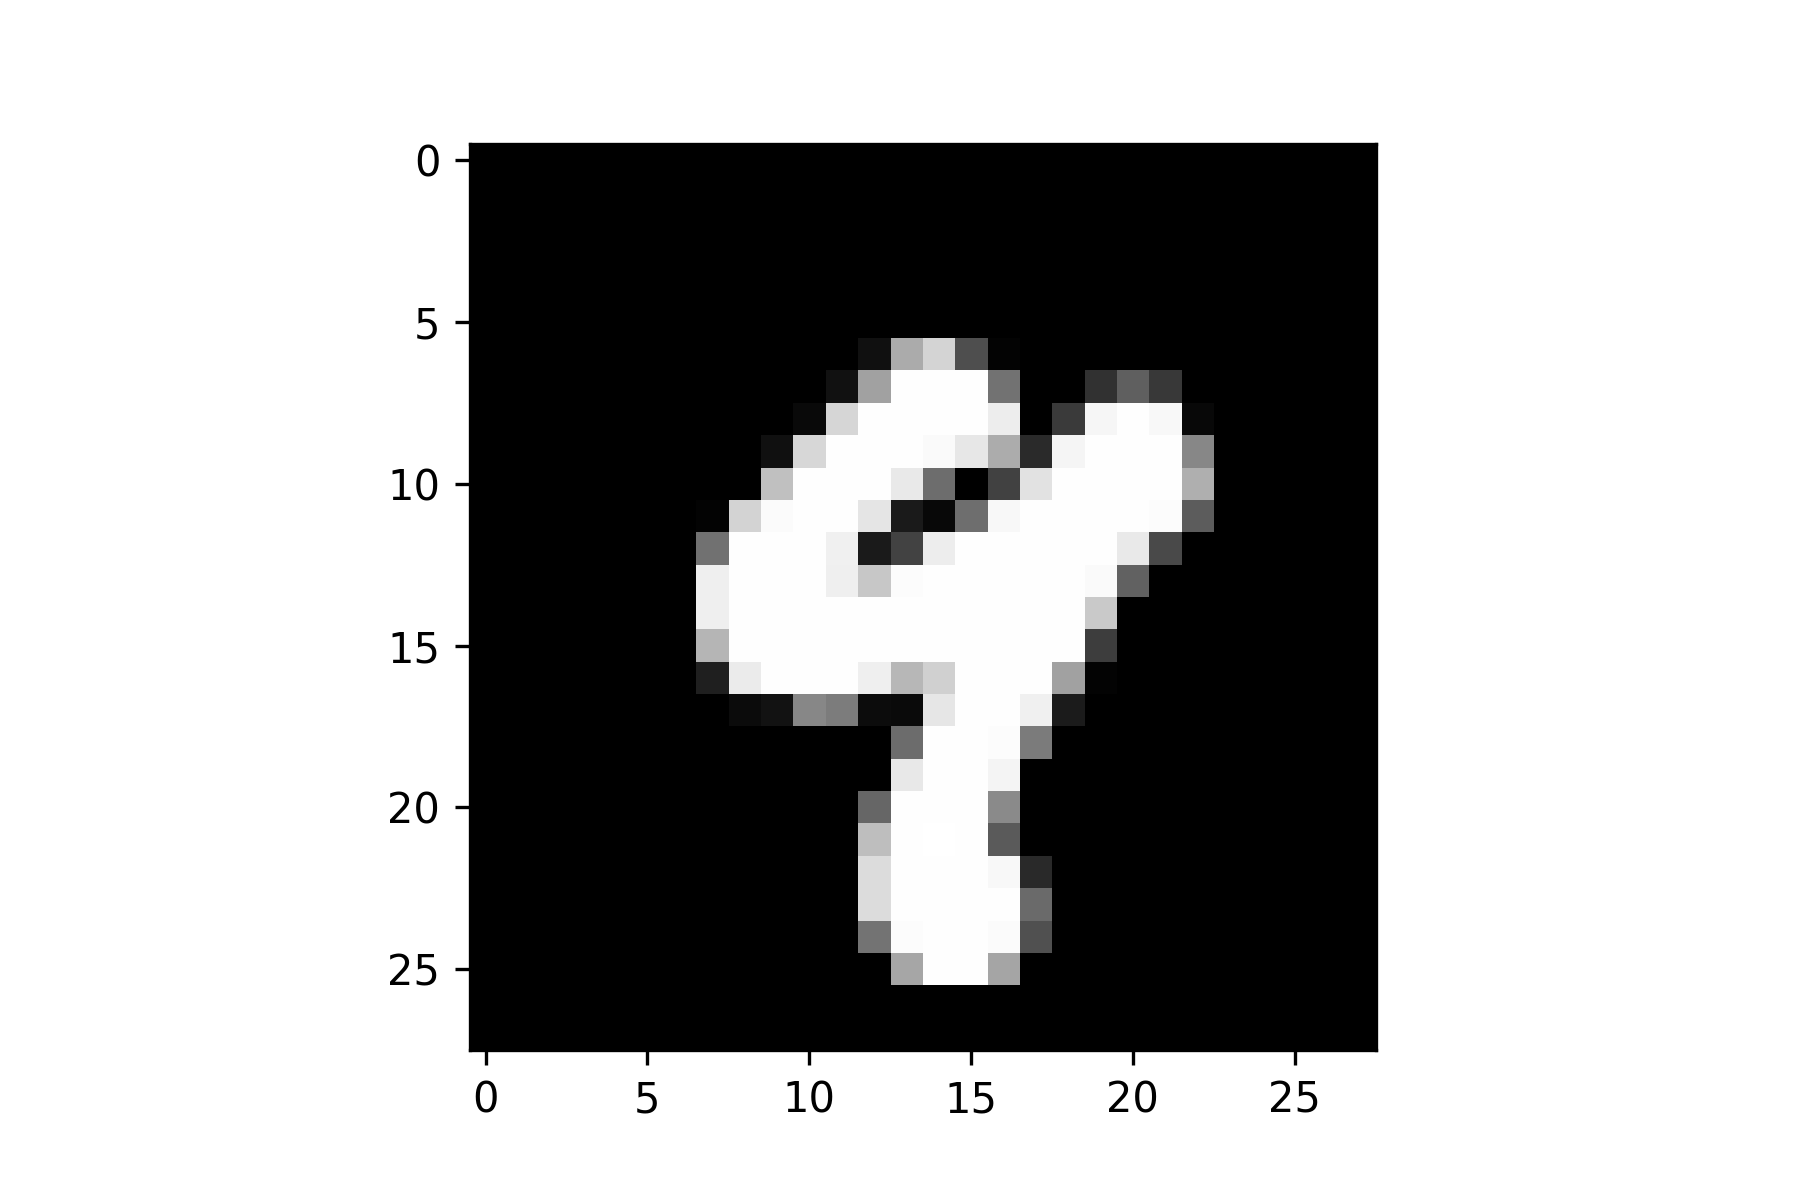
\includegraphics[width=5.0cm]{4}
        \caption{
            Real class: 7 (0.10)\\
            Predicted class: 0 (1.06)}
        \label{fig:example_2}
    \end{subfigure}
    \hfill
    % example 3
    \begin{subfigure}{0.32\textwidth}
        \centering
        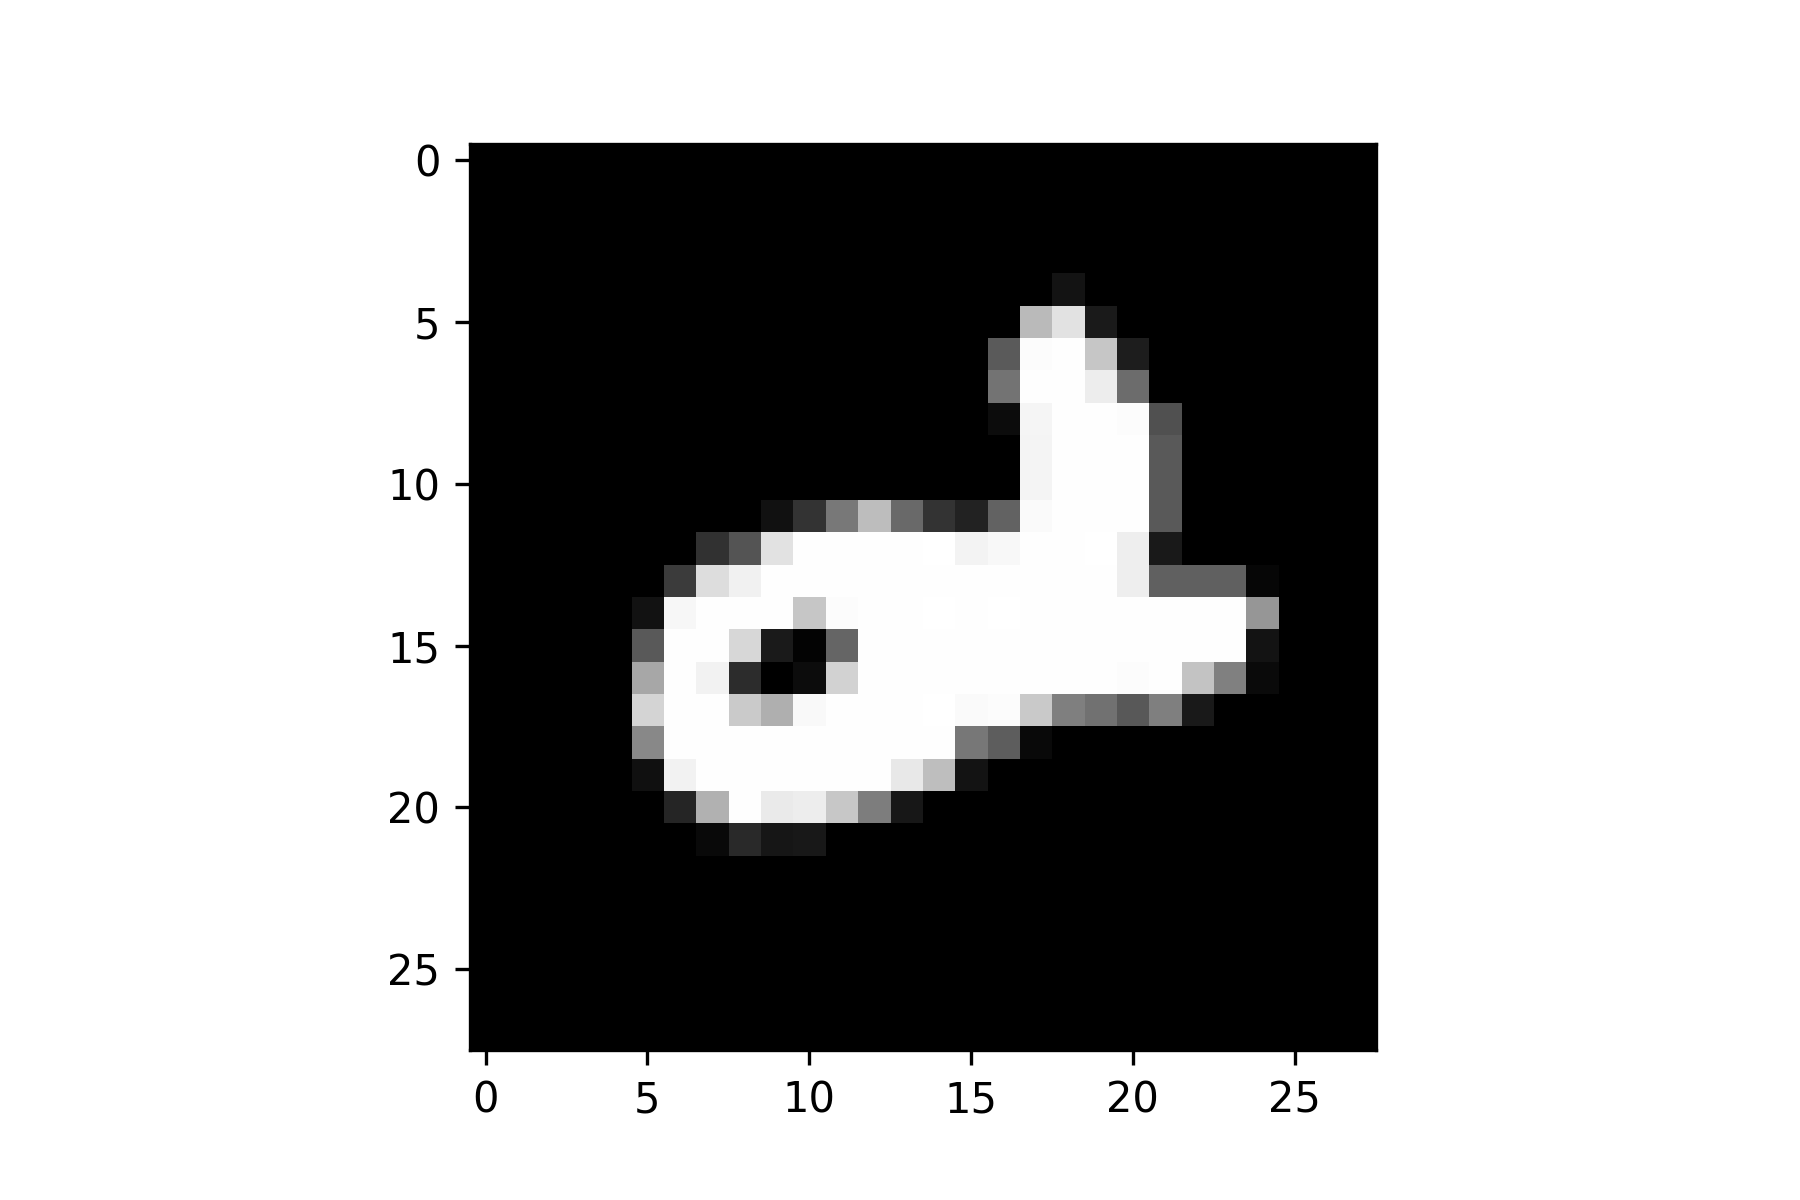
\includegraphics[width=5.0cm]{8}
        \caption{
            Real class: 4 (0.02)\\
            Predicted class: 7 (0.90)}
        \label{fig:example_3}
    \end{subfigure}
    \hfill
    % example 4
    \begin{subfigure}{0.32\textwidth}
        \centering
        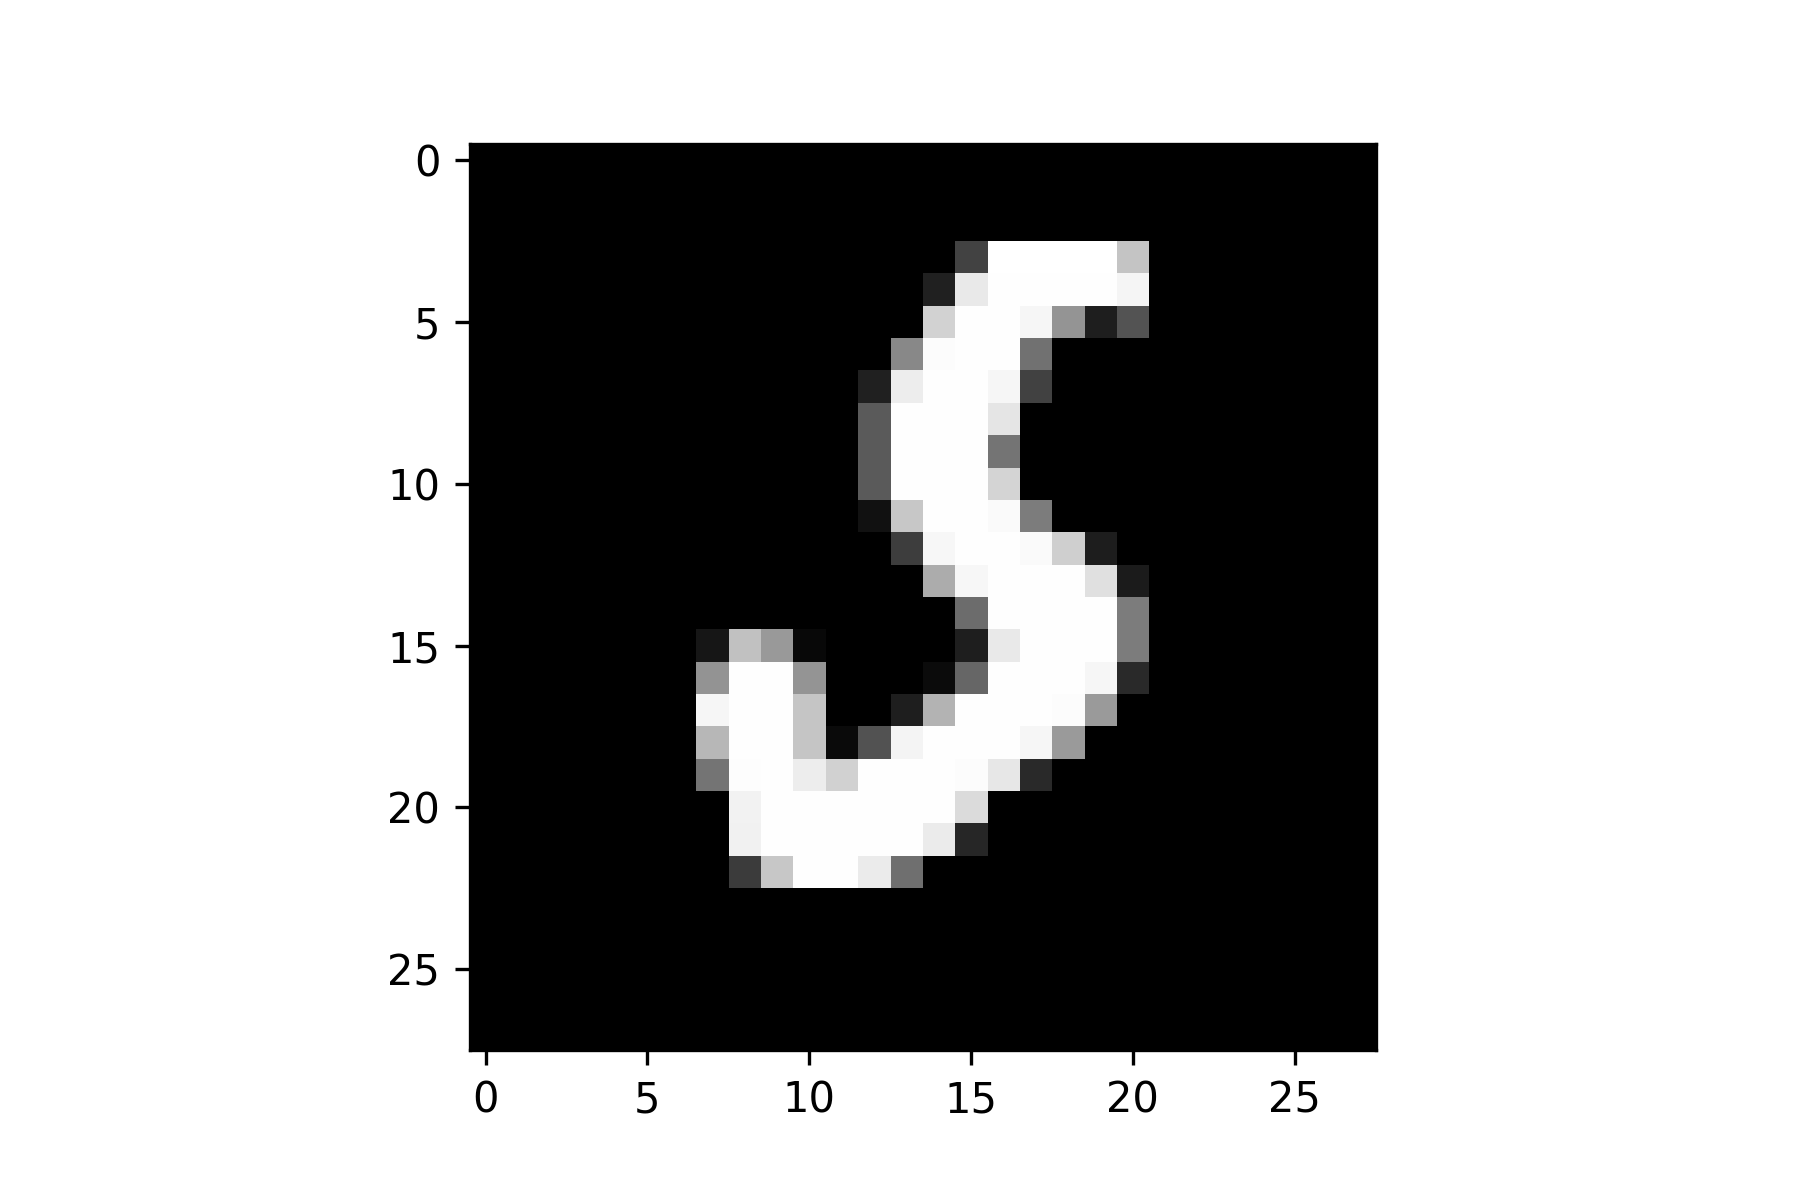
\includegraphics[width=5.0cm]{11}
        \caption{
            Real class: 9 (-0.12)\\
            Predicted class: 7 (0.73)}
        \label{fig:example_4}
    \end{subfigure}
    \hfill
    % example 5
    \begin{subfigure}{0.32\textwidth}
        \centering
        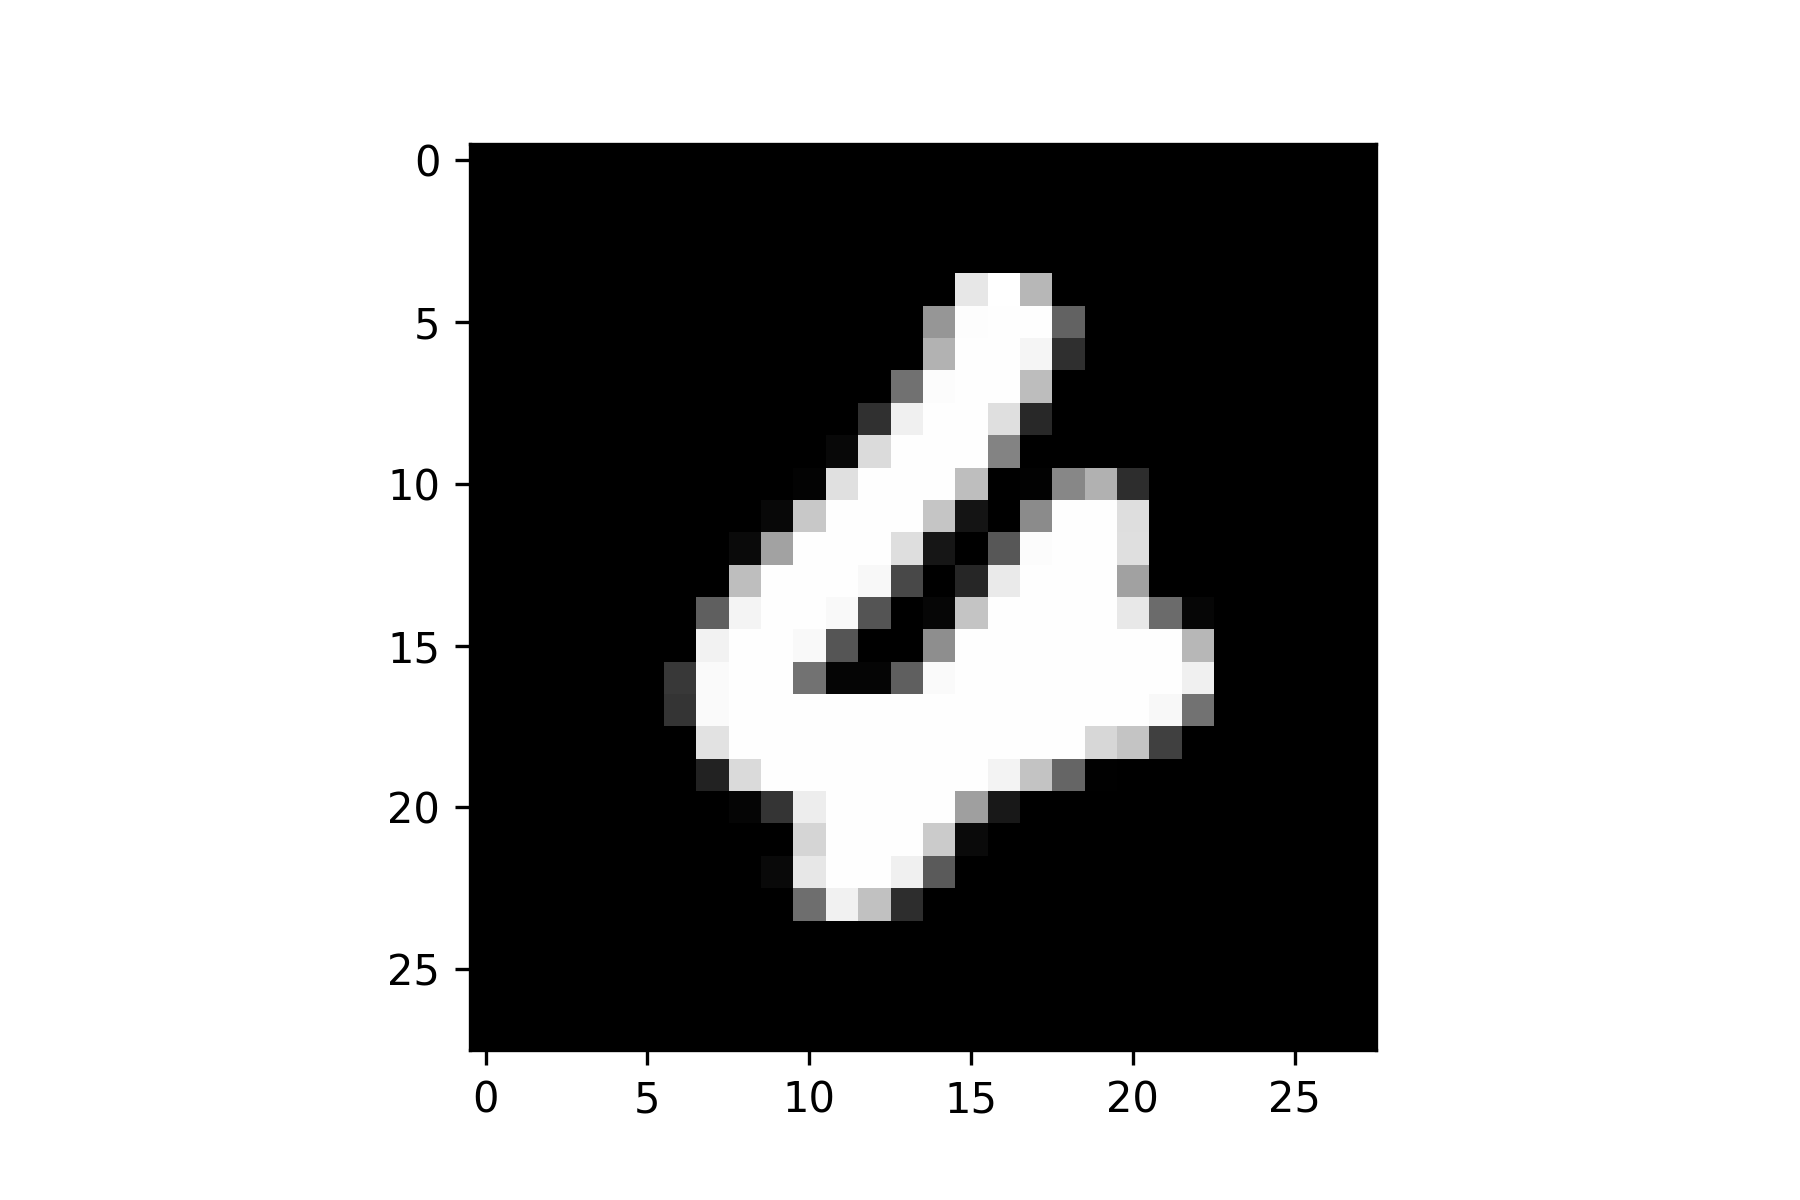
\includegraphics[width=5.0cm]{12}
        \caption{
            Real class: 5 (-0.07)\\
            Predicted class: 6 (0.78)}
        \label{fig:example_5}
    \end{subfigure}
    \hfill
    % example 6
    \begin{subfigure}{0.32\textwidth}
        \centering
        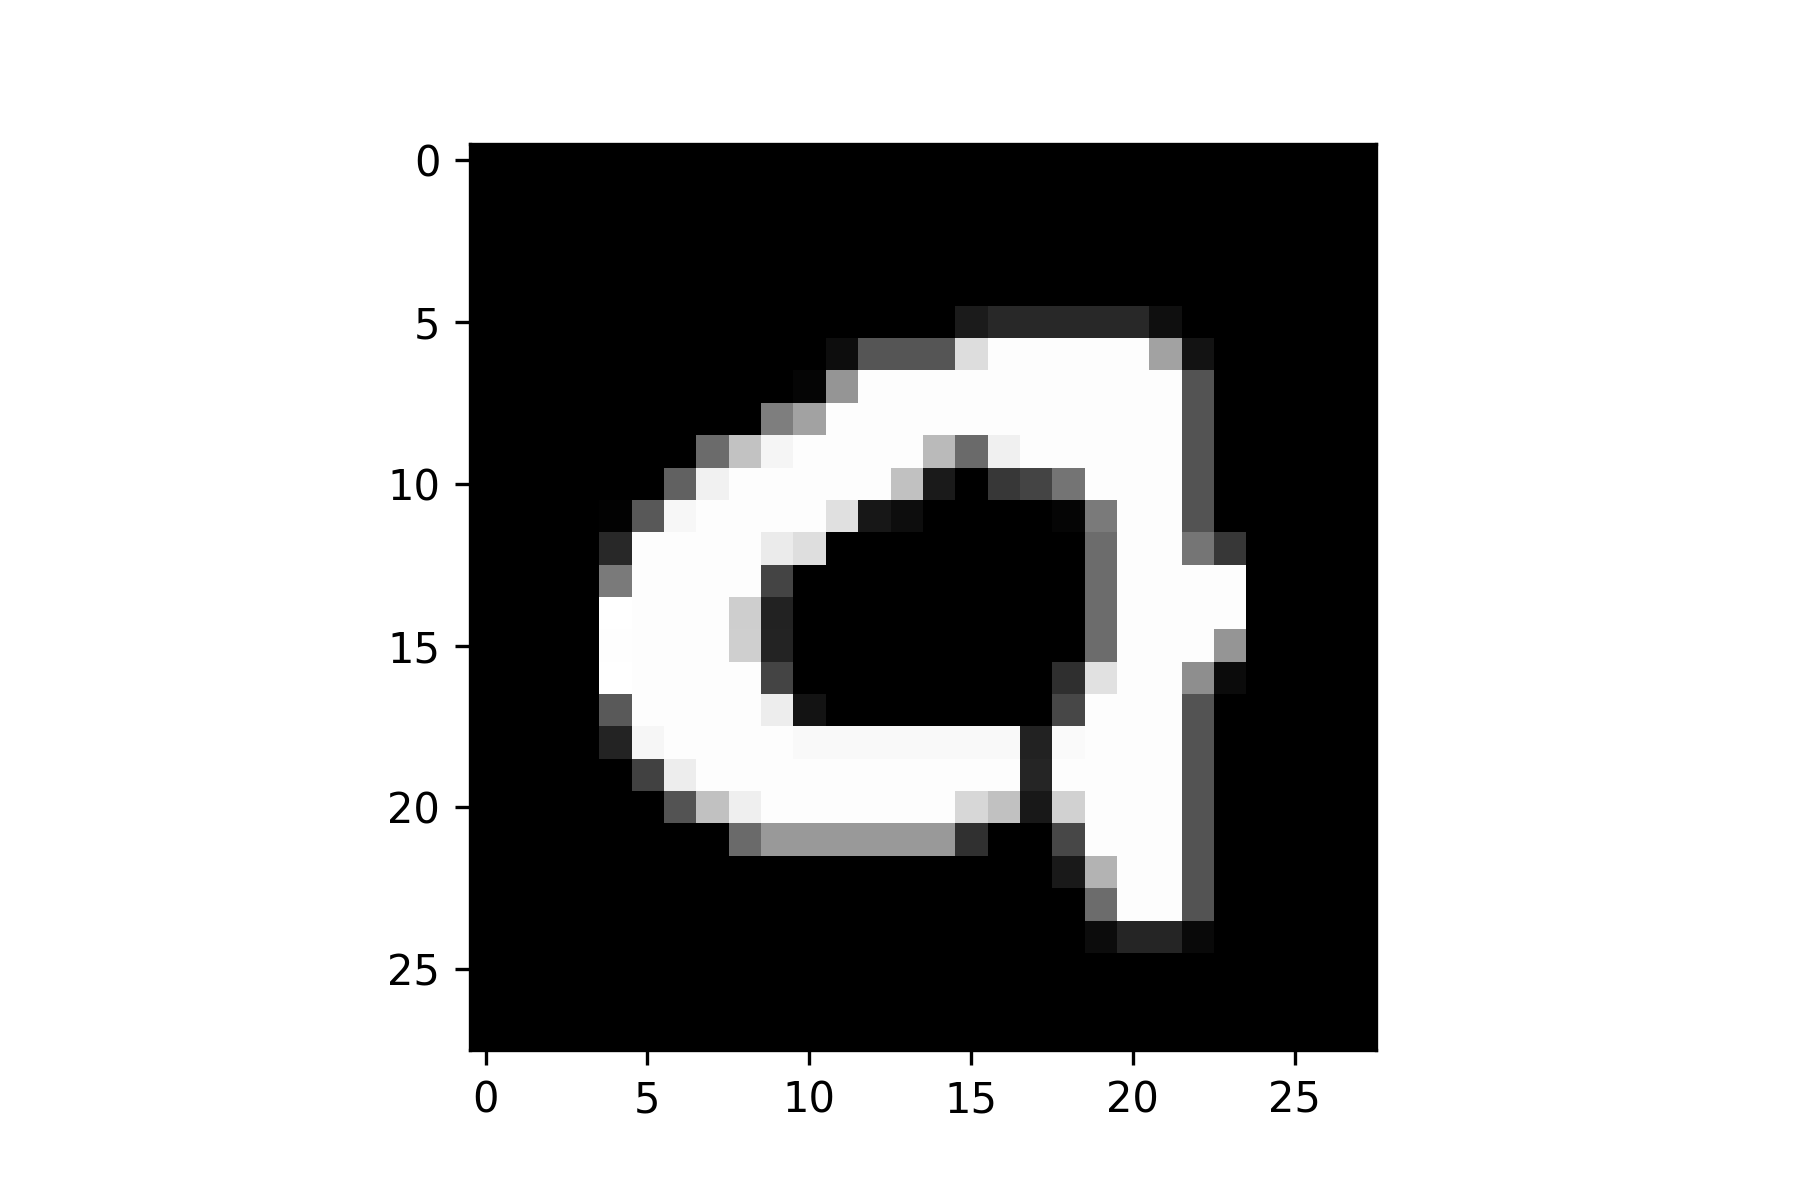
\includegraphics[width=5.0cm]{14}
        \caption{
            Real class: 4 (0.14)\\
            Predicted class: 0 (0.97)}
        \label{fig:example_6}
    \end{subfigure}
    \hfill
    % example 7
    \begin{subfigure}{0.32\textwidth}
        \centering
        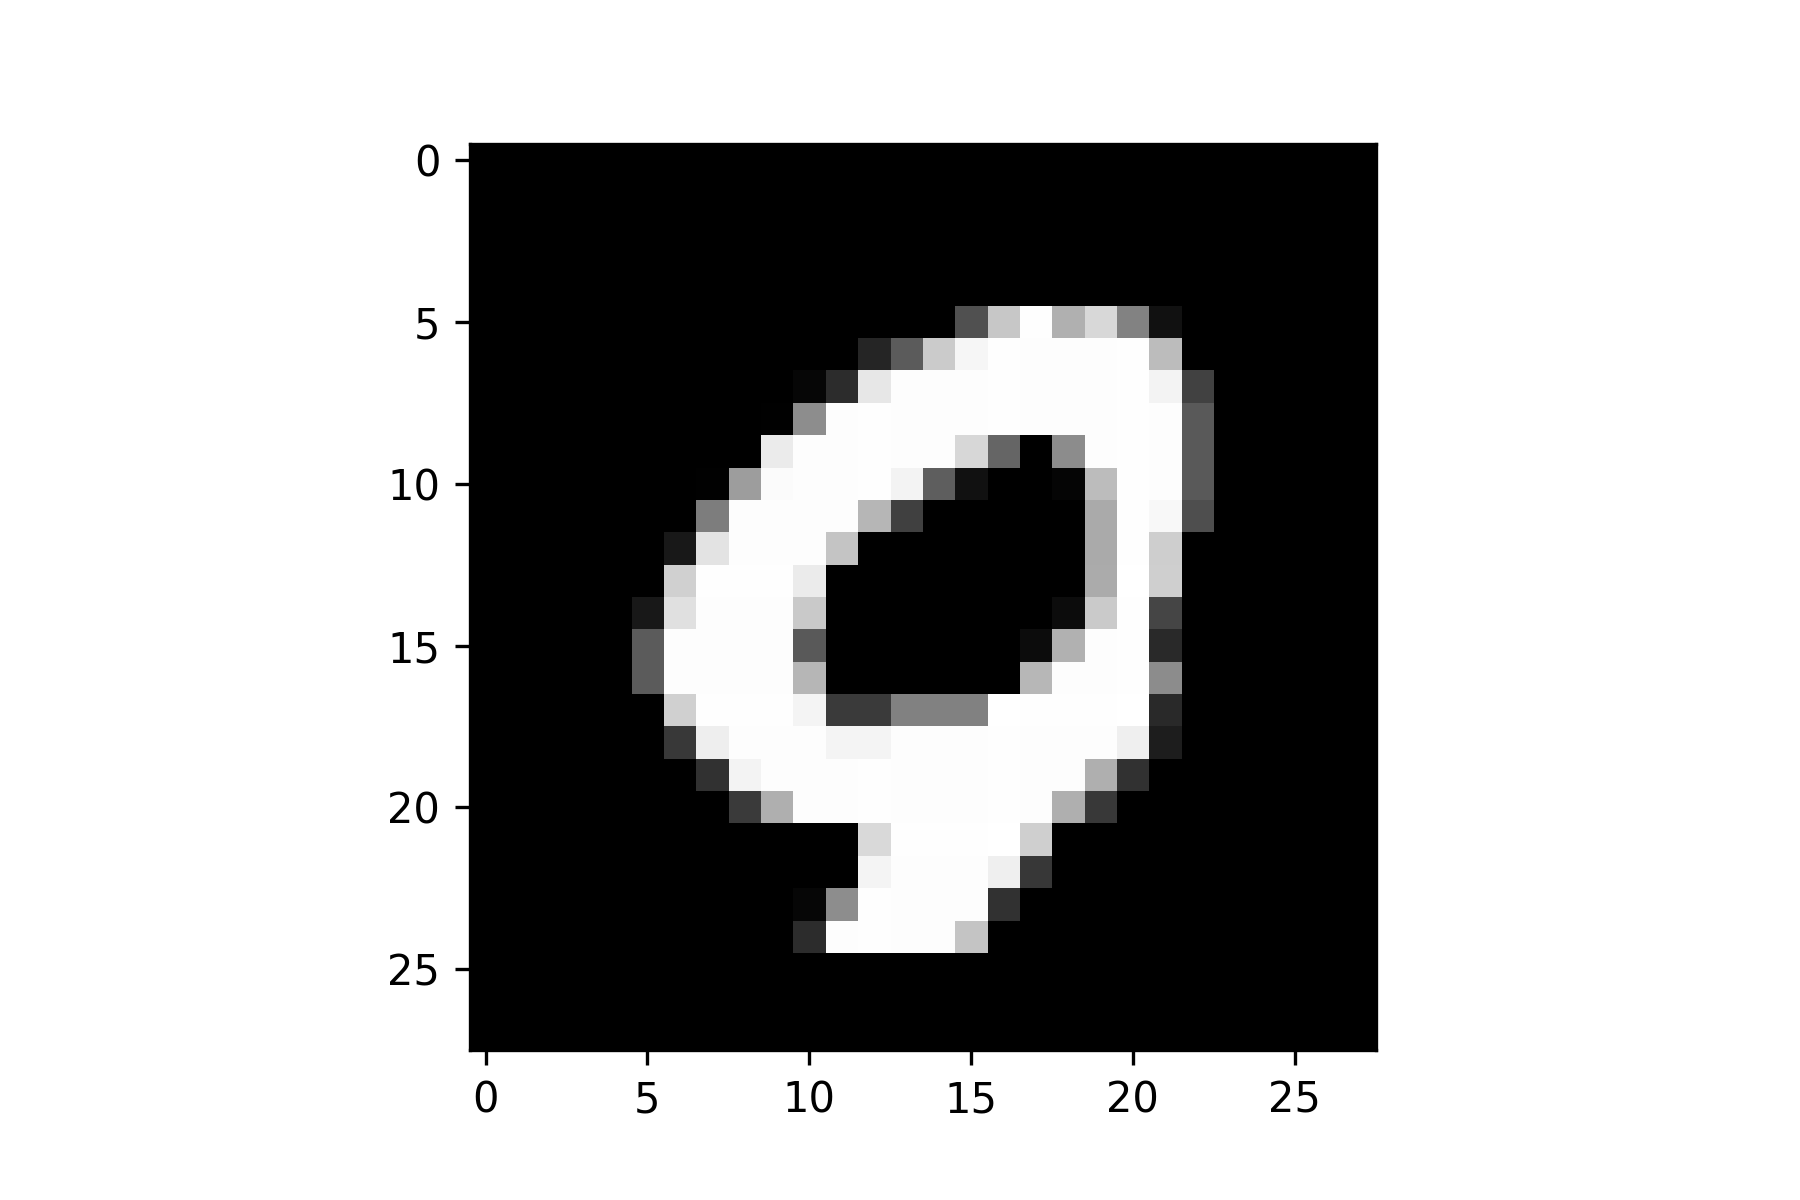
\includegraphics[width=5.0cm]{17}
        \caption{
            Real class: 9 (-0.04)\\
            Predicted class: 0 (0.77)}
        \label{fig:example_7}
    \end{subfigure}
    \hfill
    % example 8
    \begin{subfigure}{0.32\textwidth}
        \centering
        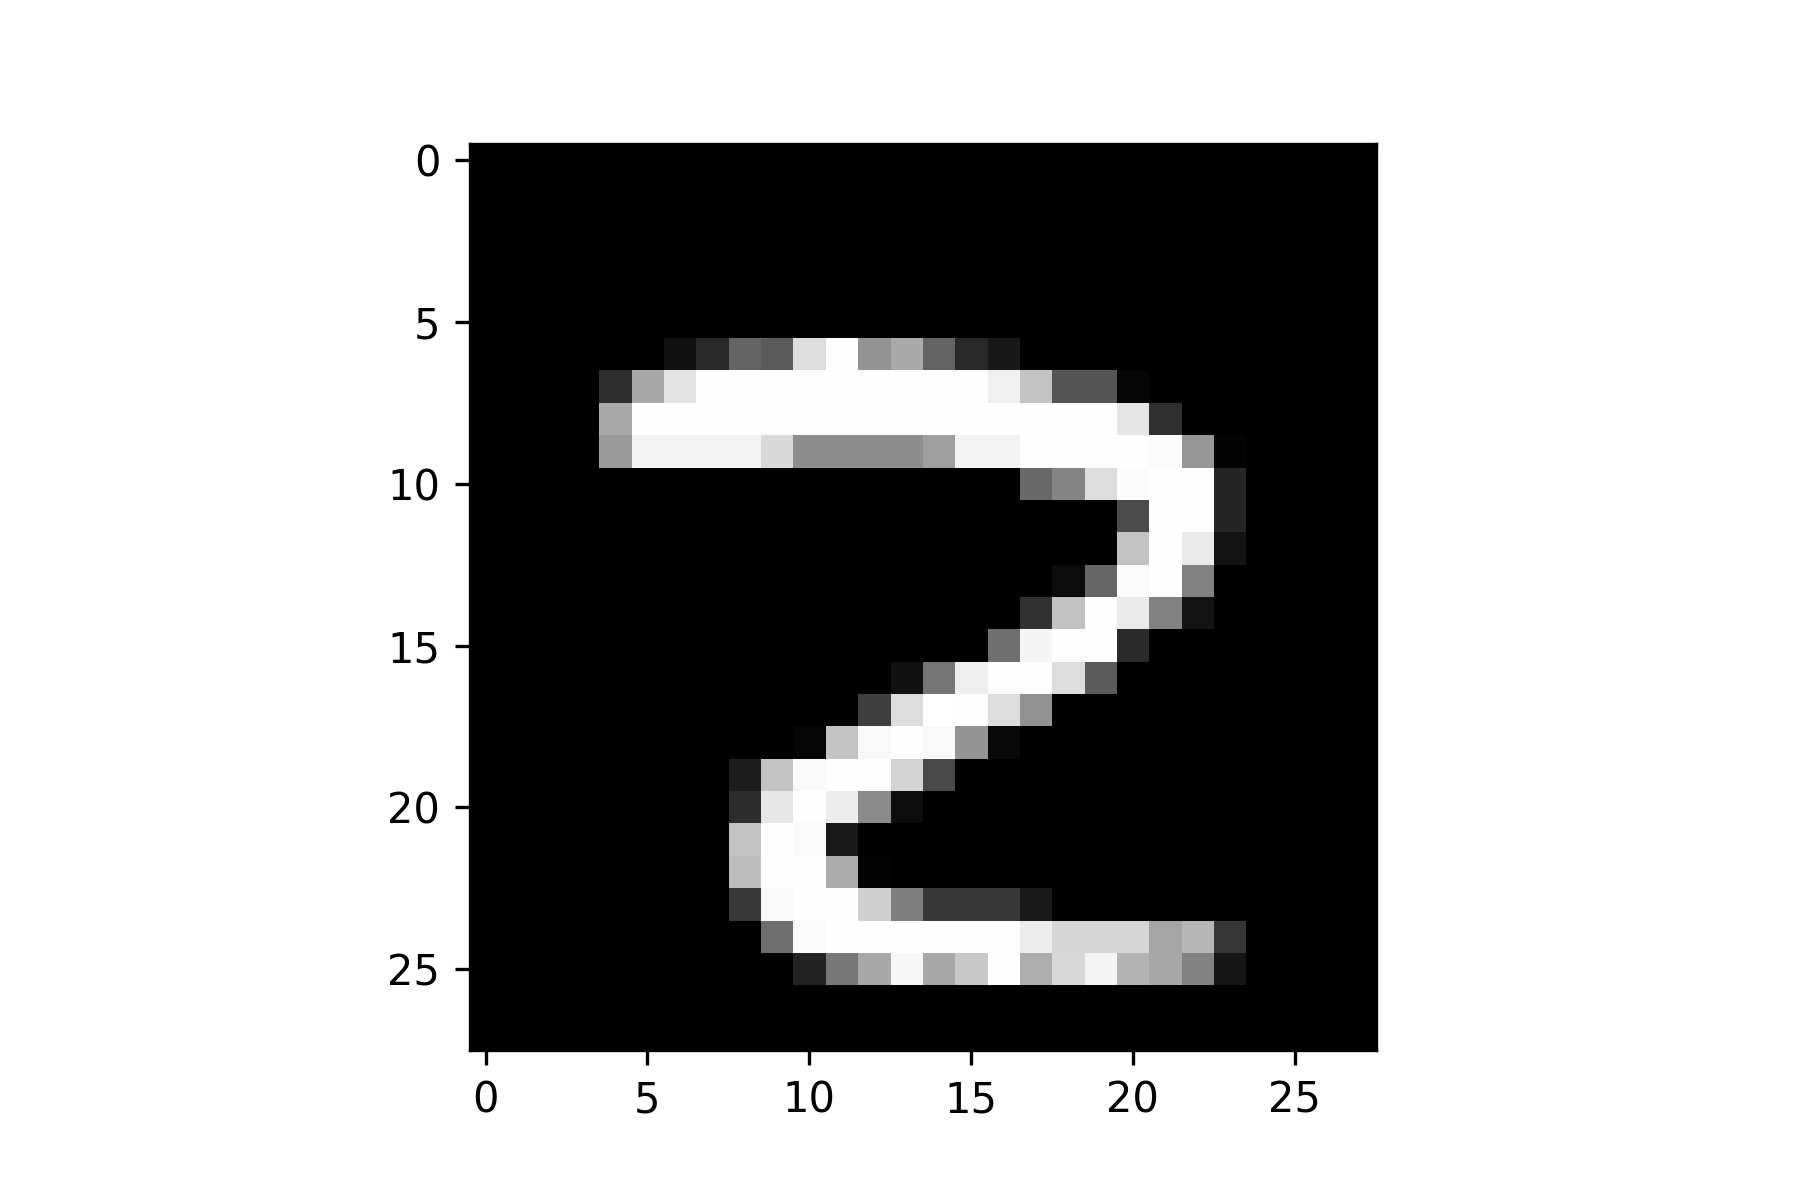
\includegraphics[width=5.0cm]{18}
        \caption{
            Real class: 1 (-0.14)\\
            Predicted class: 7 (0.66)}
        \label{fig:example_8}
    \end{subfigure}
    \hfill
    % example 9
    \begin{subfigure}{0.32\textwidth}
        \centering
        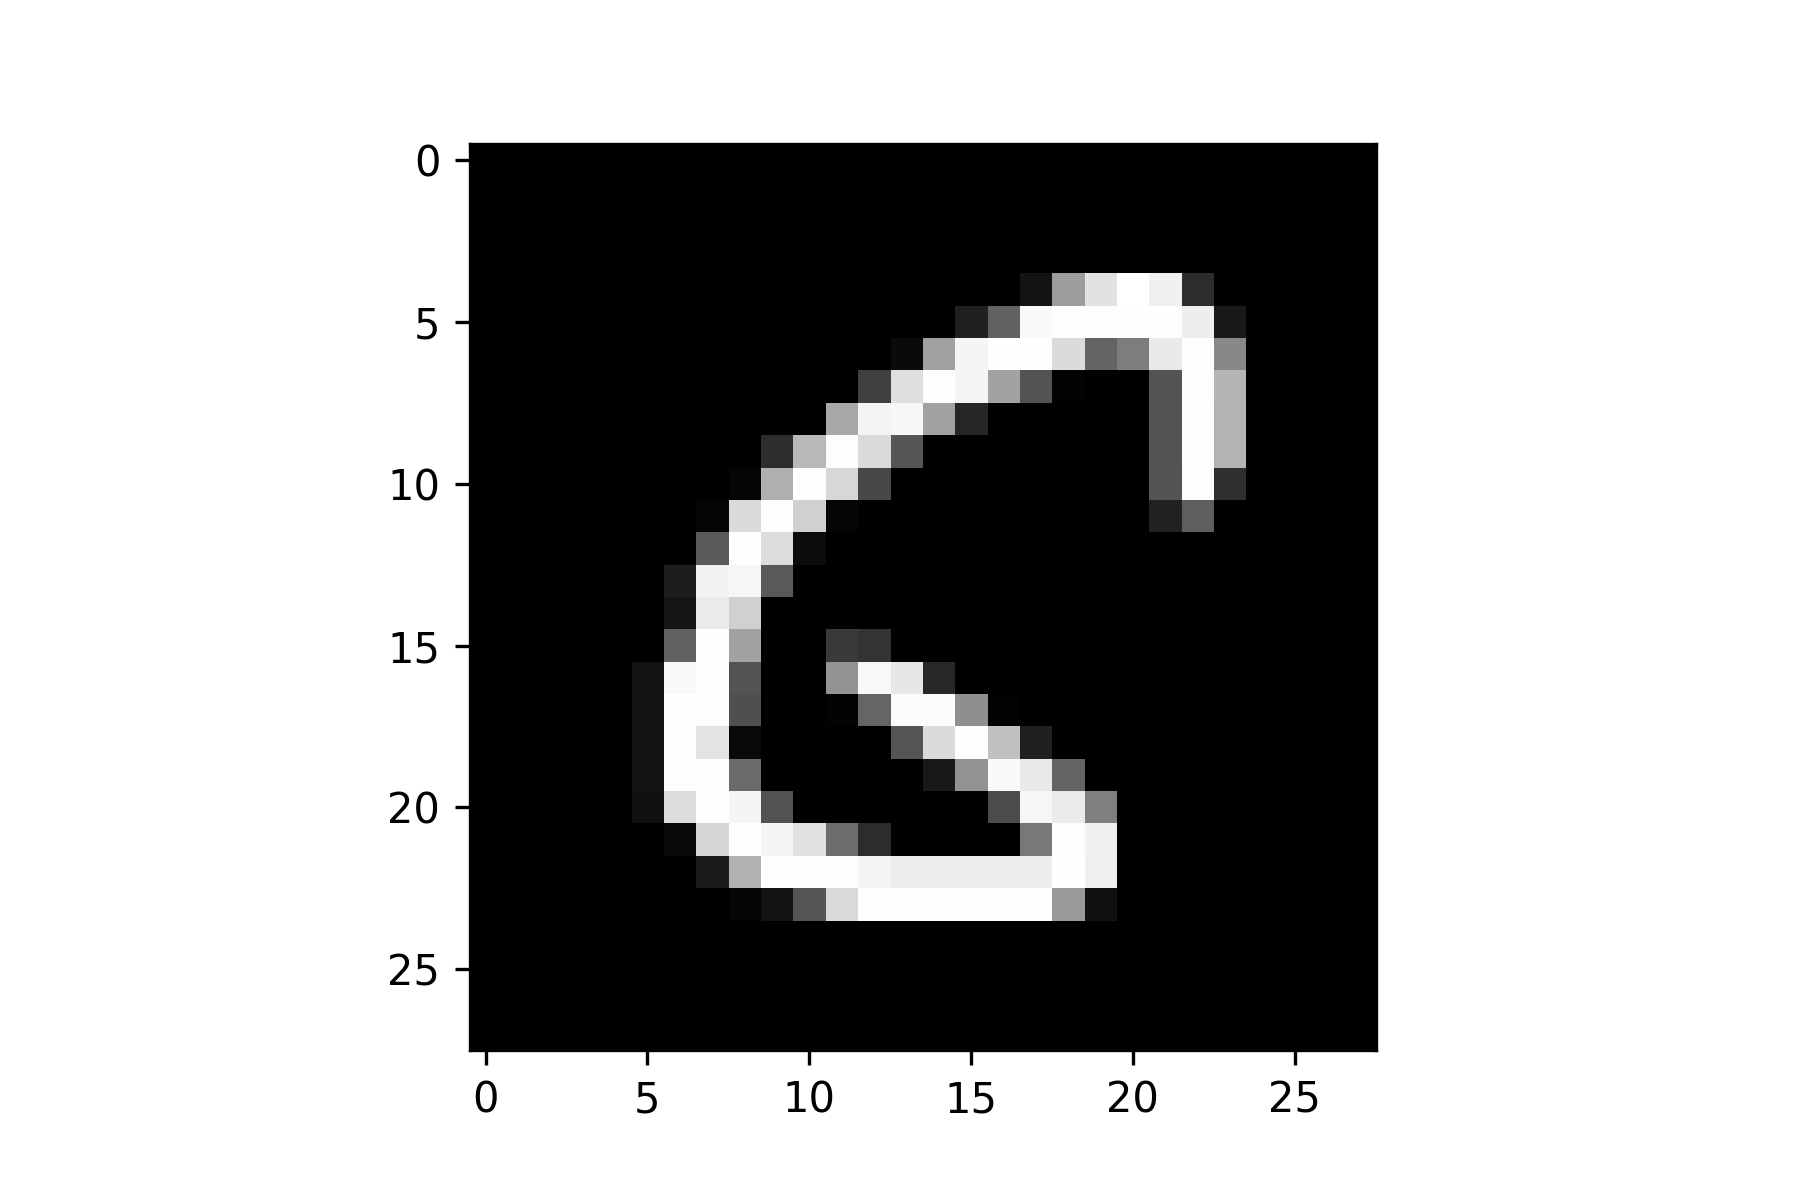
\includegraphics[width=5.0cm]{19}
        \caption{
            Real class: 3 (-0.14)\\
            Predicted class: 8 (0.66)}
        \label{fig:example_9}
    \end{subfigure}
    \hfill
    % example 10
    \begin{subfigure}{0.32\textwidth}
        \centering
        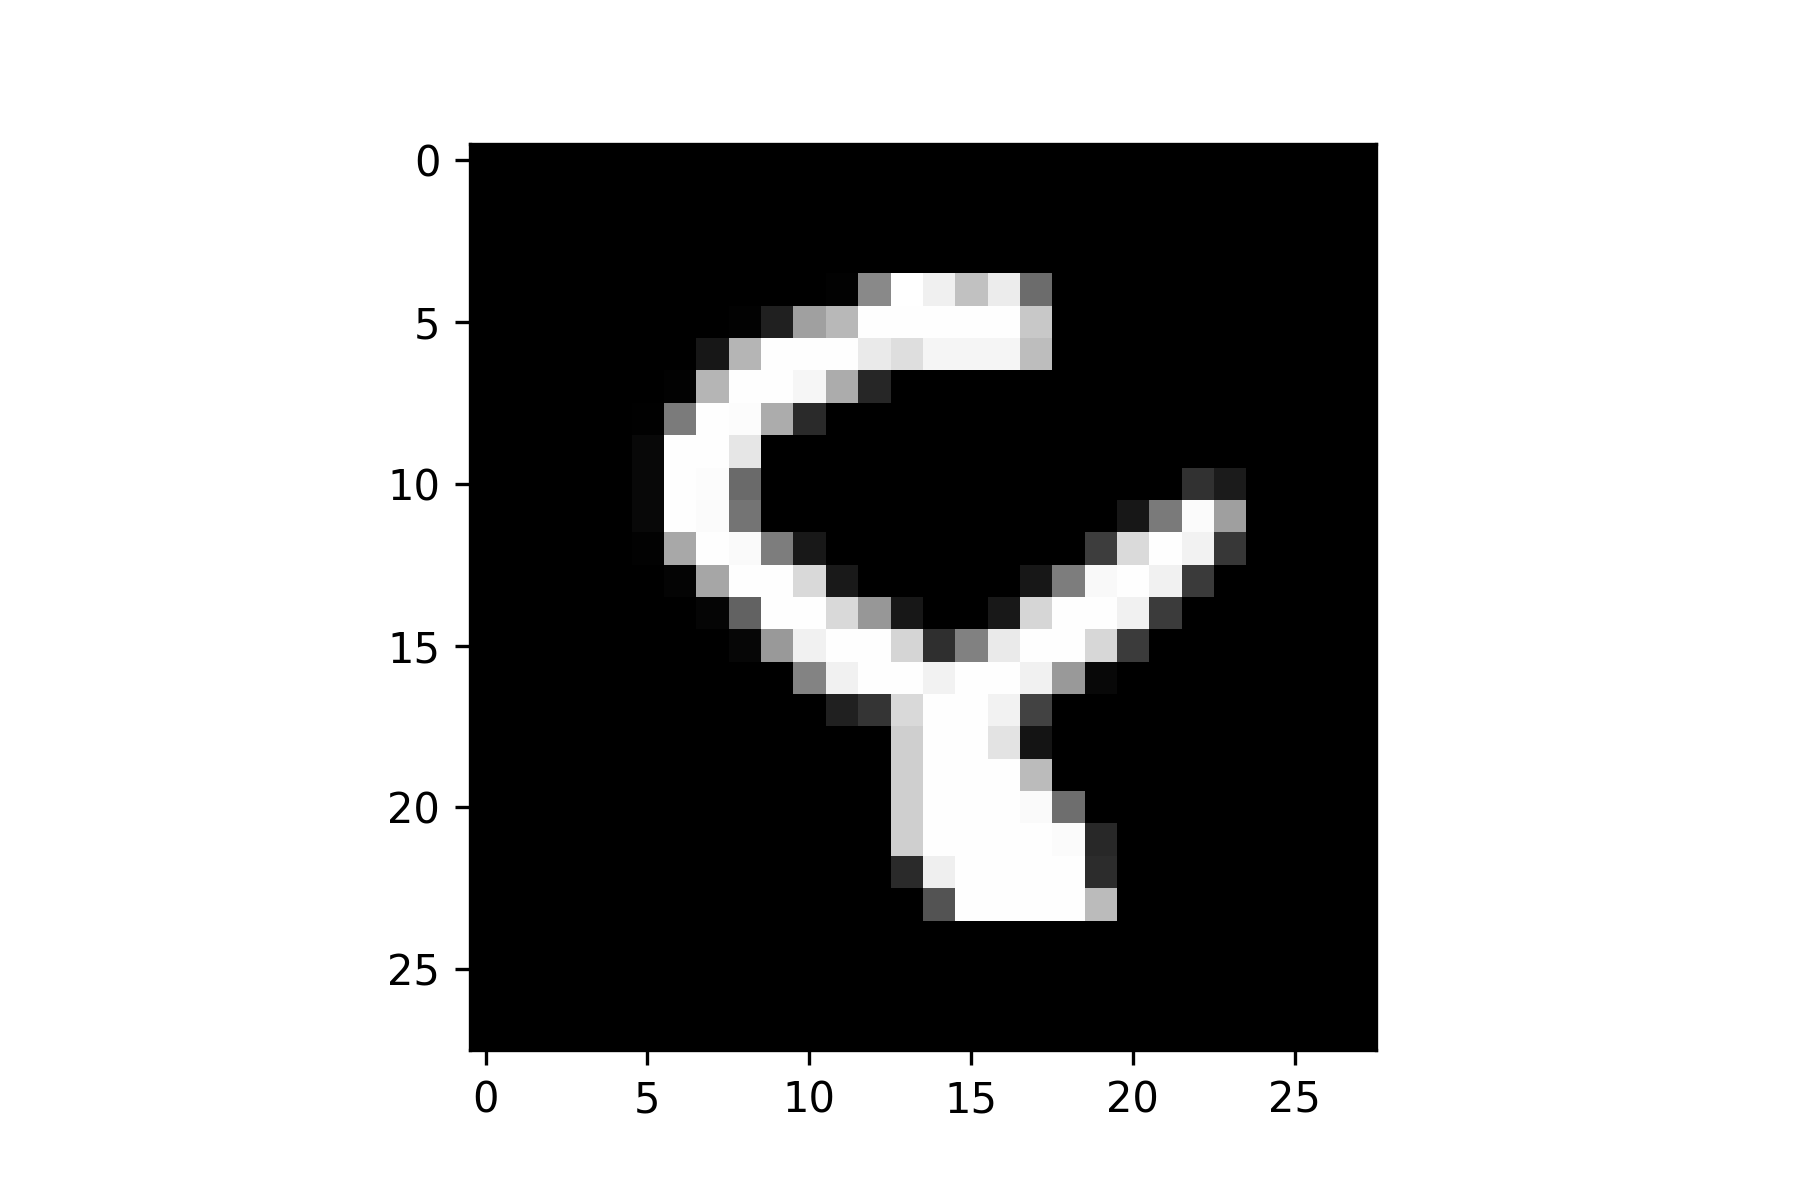
\includegraphics[width=5.0cm]{22}
        \caption{
            Real class: 8 (-0.03)\\
            Predicted class: 4 (0.74)}
        \label{fig:example_10}
    \end{subfigure}
    \hfill
    % example 11
    \begin{subfigure}{0.32\textwidth}
        \centering
        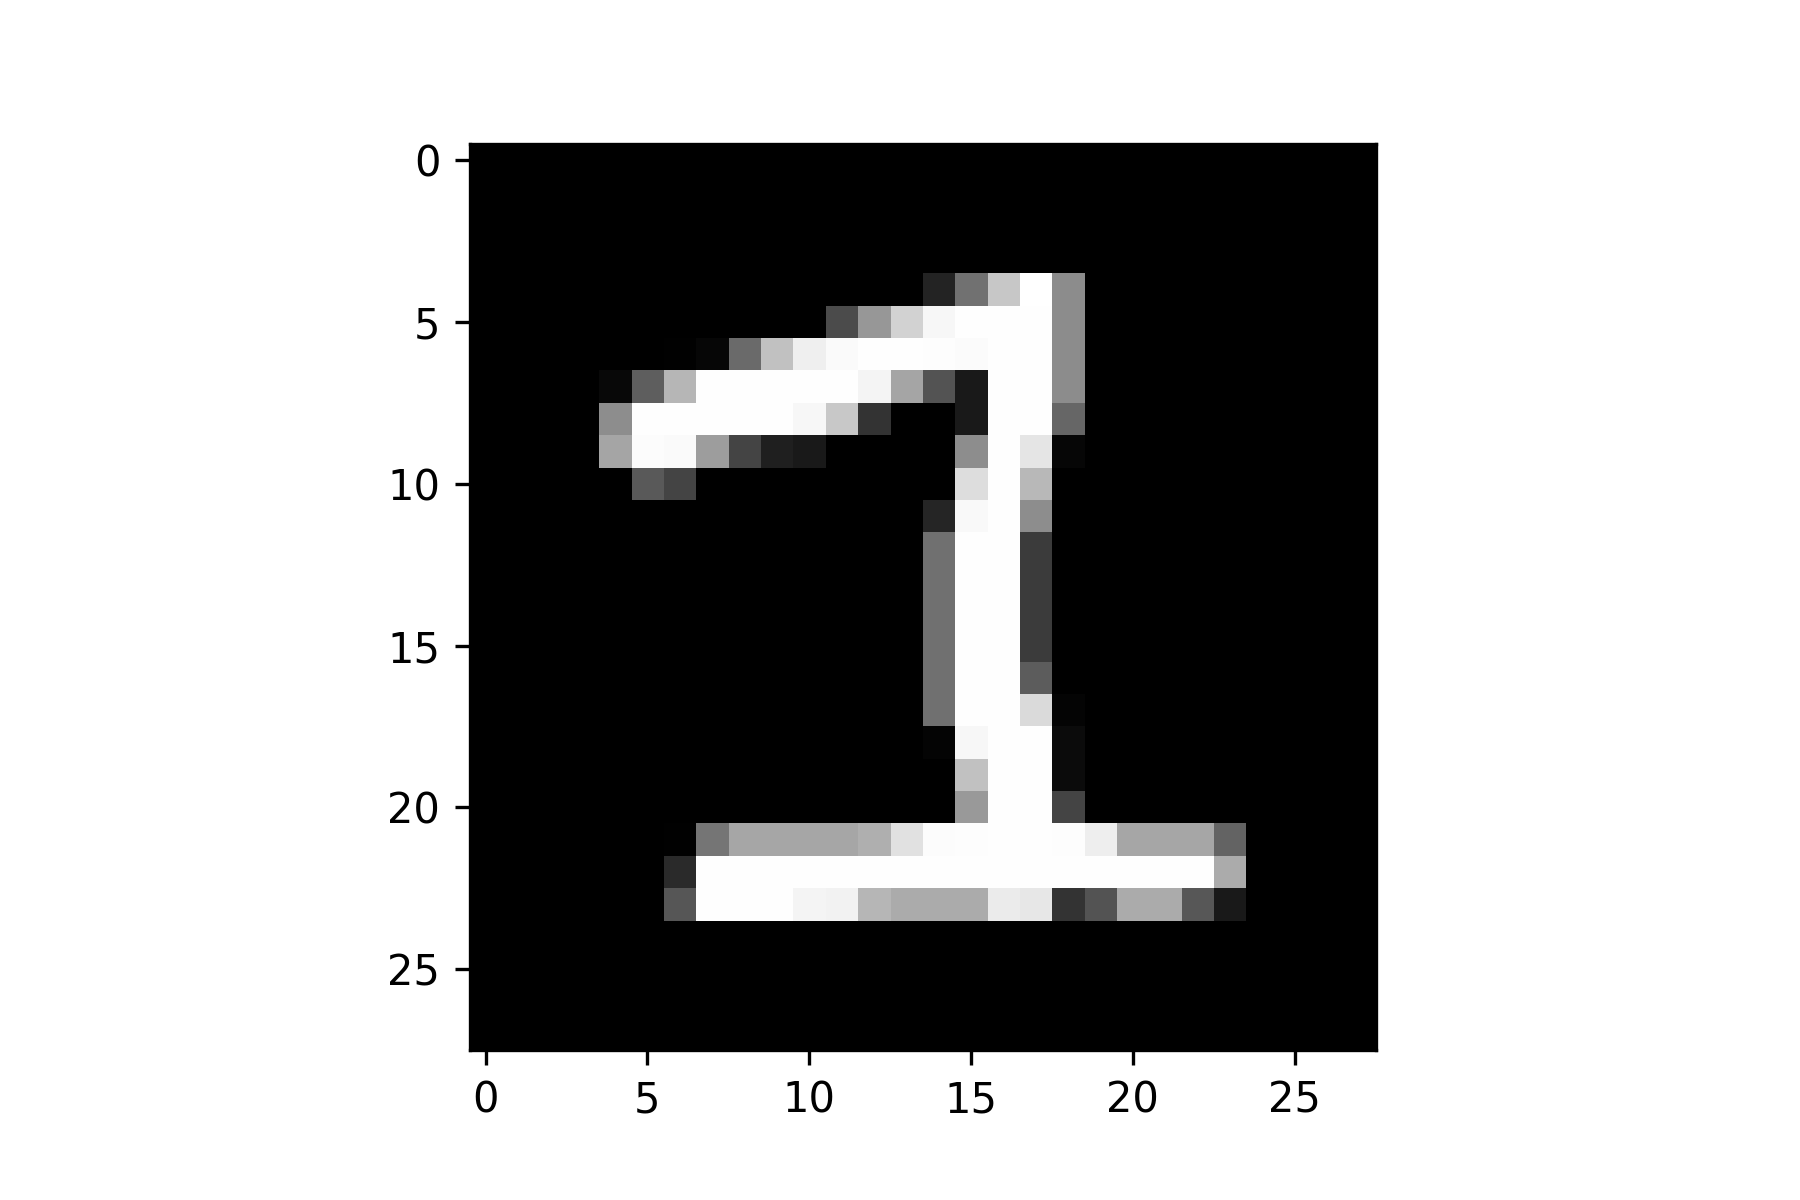
\includegraphics[width=5.0cm]{24}
        \caption{
            Real class: 5 (-0.11)\\
            Predicted class: 6 (0.65)}
        \label{fig:example_11}
    \end{subfigure}
    \hfill
     % example 12
    \begin{subfigure}{0.32\textwidth}
        \centering
        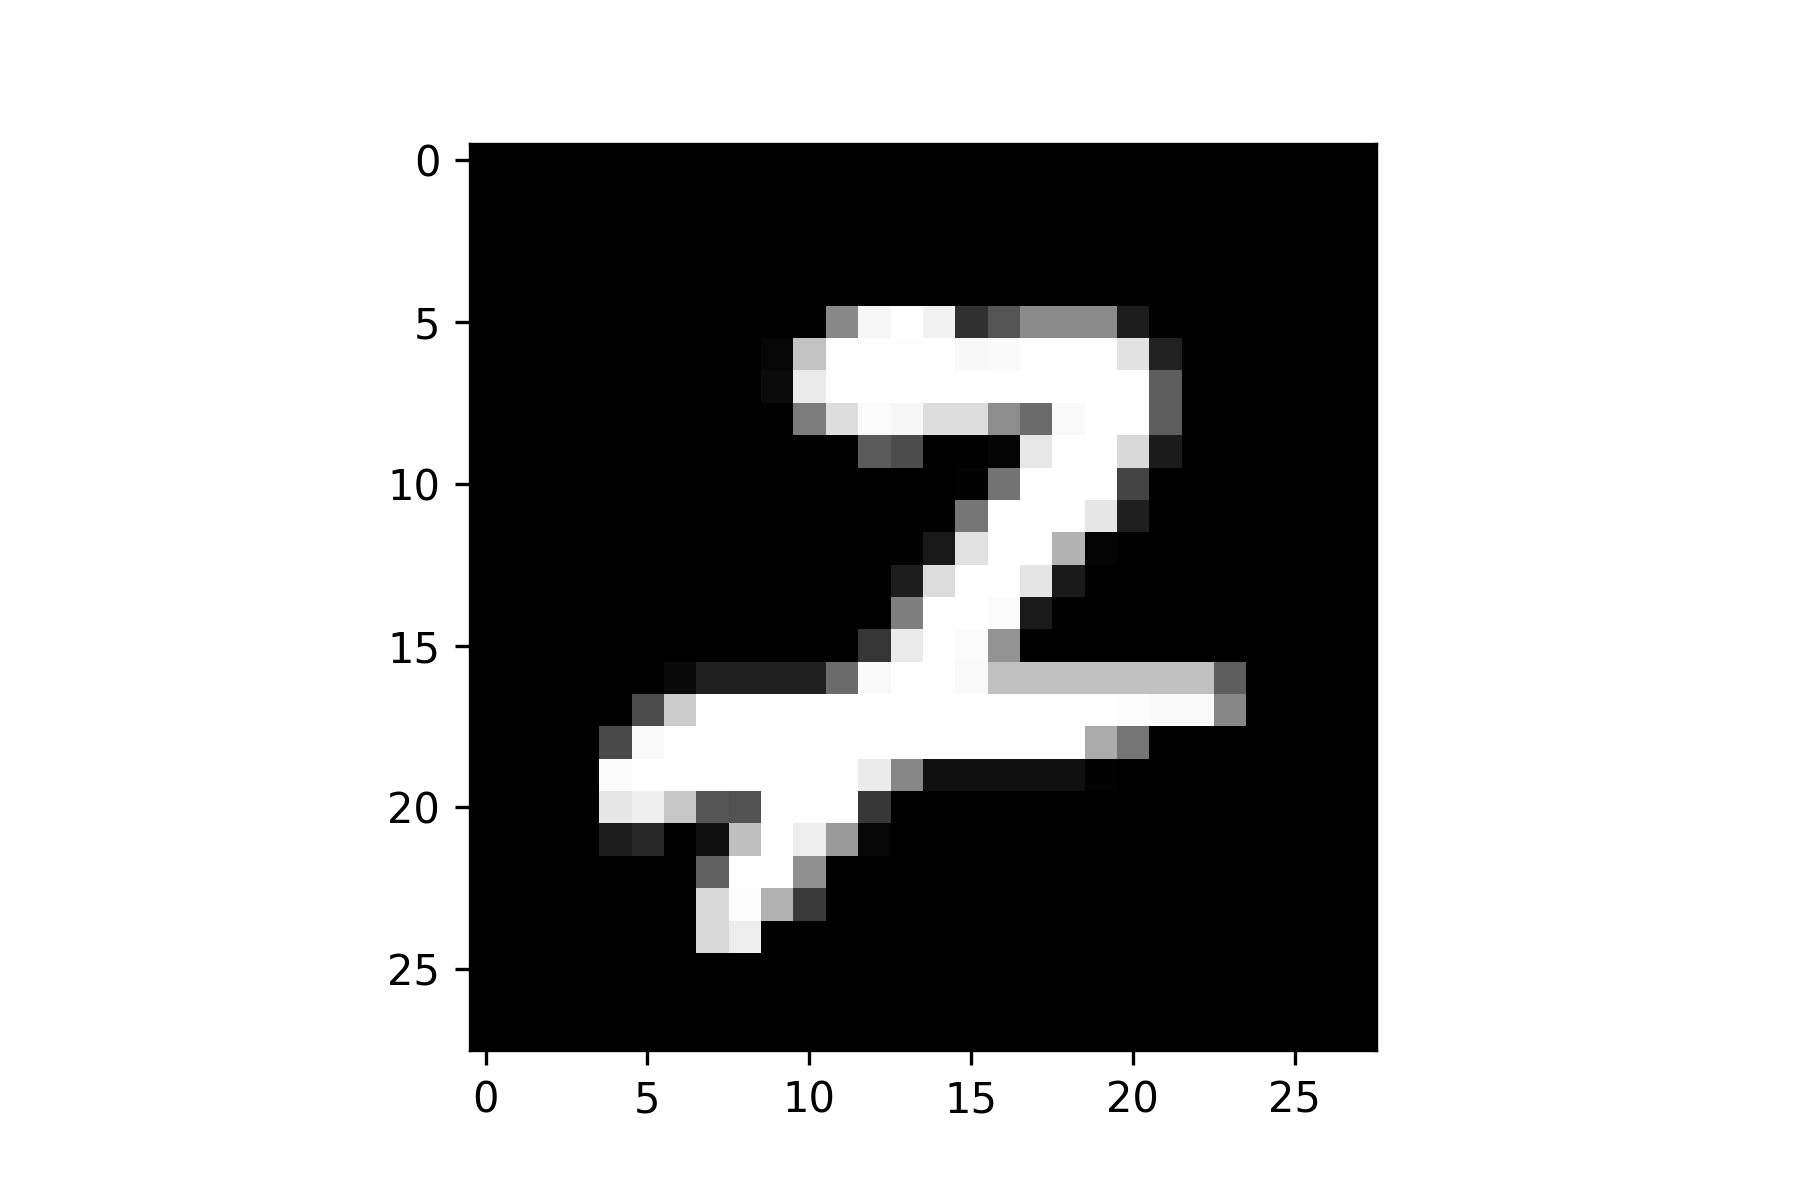
\includegraphics[width=5.0cm]{29}
        \caption{
            Real class: 6 (0.09)\\
            Predicted class: 4 (0.82)}
        \label{fig:example_12}
    \end{subfigure}
    \hfill
    % caption and label
    \caption{Misclassified digits} 
    \label{fig:misclassified_digits}
\end{figure}

\newpage

%=================================================
\subsection{Performance and computational resources improvements}
%=================================================

\textbf{Question:} \newline
Seguindo a sugestão de empregar 500 unidades na camada intermediária da rede neural, apresente argumentos para sustentar o ganho de desempenho verificado e uma execução em menor tempo computacional, quando comparado com o classificador linear da Q1.
\vspace{5mm}
%-------------------------------------------------
\textbf{\\Answer:}
\begin{itemize}
    \item \underline{Performance improvement:}\vspace{5pt}\\
        We can see better results using the ELM comparing to the linear model of Q1 because now we use a non-linearity activate function at the hidden layer (here we used the rectifier activation function, i.e., the units of the hidden layer are ReLUs). The universal approximation theorem states that a feed-forward network with a single hidden layer with a finite number of neurons with non-linear activation function is capable of approximate any continuous function. Even though we are not training a neural network, but using ``ready-to-use" hidden layer weights instead, the intuition behind the non-linear layer followed by a linear layer is the same. We can also see this performance improvement at the perspective that instead of finding a classifier directly from the values of the pixels in the image, now we have a new problem to solve. Now we have to find a classifier using the outputs of the neurons in the hidden layer, which is an easier problem than the previous one.

    \item \underline{Computational resources improvement:}\vspace{5pt}\\
    The reason that the code from Q2 runs faster than the code from Q1 is that the operation with the highest computational cost is by far calculating the inverse matrix of $(X^T X + \lambda I')$ when computing the weights, as can be seen in the following equation:
    \[{\textbf{W} = (X^T X + \lambda I')^{-1} X^T \textbf{y}}\]
    In Q1 we need to invert the matrix $(X^T X + \lambda I')$ of size 785 x 785, while in Q2 we have to invert the matrix $(H^T H + \lambda I')$ of size 501 x 501. This difference of shapes considering the matrix inversion is decisive to lower the computational time, even though in Q2 there is an extra product $H = X W'$ happening before the calculus of the \textbf{W} matrix, where $W'$ is the matrix with the weights of the hidden layers chosen randomly.\\
    When using the rectifier activation function (commonly called ReLU, although ReLU is the unit - neuron), some of the outputs of the hidden layer will be zero. This might make the product of $H^T H$ a bit easier since a portion of elements will be zero, but the dominant term where most of the complexity resides is definetely at the computation of the inverse matrix.
\end{itemize}

\newpage

%=================================================
\subsection{Regularization coefficients comparison (Linear and ELM)}
%=================================================

\textbf{Question:} \newline
Compare os coeficientes de regularização obtidos nessas duas primeiras atividades (classificador linear da Q1 e ELM da Q2), os apresentando numa única tabela para fácil visualização, e procure justificar a diferença. 
%-------------------------------------------------

\textbf{\\Answer:}\\
The regularization coefficients for both Q1 and Q2 (coarse and fine search) can be seen in Table \ref{tab:alpha_comp}.

\begin{table}[H]
    \begin{center}
        \begin{tabular}{r|c|c|c|c|}
            \cline{2-5}
            & \multicolumn{4}{|c|}{\cellcolor[gray]{0.8}{$\lambda$ optimum}} \\
            \cline{2-5}
            & \multicolumn{2}{|c|}{\cellcolor[gray]{0.8}{Q1}} & \multicolumn{2}{|c|}{\cellcolor[gray]{0.8}{Q2}} \\
            \cline{2-5}
            & \cellcolor[gray]{0.8}{MSE} & \cellcolor[gray]{0.8}{Accuracy} & \cellcolor[gray]{0.8}{MSE} & \cellcolor[gray]{0.8}{Accuracy} \\
            \cline{1-5}
            \multicolumn{1}{|r|}{\cellcolor[gray]{0.8}{coarse search}} & 64   & 1024   & 64   & 256   \\
            \cline{1-5}
            \multicolumn{1}{|r|}{\cellcolor[gray]{0.8}{fine search}}   & 51.5 & 1091.8 & 102.7 & 662.7 \\
            \cline{1-5}
        \end{tabular}
    \end{center}
    \caption{Values of regularization coefficient found in coarse and fine searches in both Q1 and Q2}
    \label{tab:alpha_comp}
\end{table}

From now on the regularization coefficient will be just called ``alpha" to simplify the text.
%
\paragraph{The results shown in Table \ref{tab:alpha_comp} are curious, since the optimum alpha increased for the MSE criterion, but decreased for the accuracy metric. A higher value of alpha indicates that the weights are being more regularized, suggesting that the model is more flexible.}
%
\paragraph{Talking about the ELM in specific, although the results obtained are much better than the linear approach (~95\% against ~85\% of accuracy), the machine is not necessarily ``more flexible" in the sense stated in the previous paragraph. The improvements are achieved mainly because of the non-linearity activation function (tanh, ReLU) than due to flexibility, since the weights of the hidden layer were randomly chosen.}
%
\paragraph{The smaller optimum alpha for the accuracy metric suggests a less flexible model for the ELM approach when comparing to the linear model. This can be explained due to the reduced values reaching the output layer (501 vs 785) and also the quality of these signals to perform the linear classification.}
%
\paragraph{However, the bigger optimum alpha for the MSE criterion suggests that for these randomly generated weights, the ELM ended with a more flexible model than the linear one, even for a reduced number of signals reaching the linear output classifier layer.}

\newpage

%=================================================
\subsection{Regularization coefficient for a different initialization}
%=================================================

\textbf{Question:} \newline
Mantendo a mesma partição entre conjuntos de treinamento e validação, o que você espera que ocorra com o coeficiente de regularização caso os neurônios da camada intermediária sejam inicializados com pesos sinápticos distintos a cada execução? 

%-------------------------------------------------
\textbf{\\Answer:}
\paragraph{As already explained at the answer of the previous question, the flexibility of the model strongly depends on the weights of the hidden layer. By randomly choosing the weights and knowing that the role of the regularization coefficient is to prevent overfitting in a model that is too flexible, the alpha will likely change every time, since for each weights configuration we are dealing with a new problem to solve, looking at the perspective of the output linear layer. The ``ReLU" activation function can also perform a role here, since a portion of the outputs of the hidden layer will be zero depending on the weights generated (and also the input data).}
%
\paragraph{In summary, for each randomly generated weights, a new model with a new flexibility will be generated, and depending on the flexibility, more or less regularization will be necessary. Furthermore, as stated at the answer of the previous question, the necessity of regularize the weights of the linear output layer more or less can also change when looking at the accuracy metric or the MSE criterion.}

%=================================================
\subsection{Modifications aiming better results}
%=================================================

\textbf{Question:} \newline
Promova algum tipo de alteração nas especificações da ELM e/ou de seu treinamento de modo a produzir resultados superiores àqueles conquistados ao se seguir o roteiro desta questão. Descreva adequadamente as alterações realizadas.

%-------------------------------------------------
\textbf{\\Answer:}
\paragraph{Changing the number of neurons at the hidden layer from 500 to 1000 improved the results, as shown in Table \ref{tab:elm_improved}.}

\begin{table}[H]
    \begin{center}
        \begin{tabular}{r|c|c|} 
            \cline{2-3}
            & \multicolumn{2}{|c|}{\cellcolor[gray]{0.8}{Accuracy}} \\
            \cline{2-3}
            & \cellcolor[gray]{0.8}{Training set} & \cellcolor[gray]{0.8}{Test set} \\
            \cline{1-3}
            \multicolumn{1}{|r|}{\cellcolor[gray]{0.8}{500 neurons}}  & 0.9175 & 0.9194   \\
            \cline{1-3}
            \multicolumn{1}{|r|}{\cellcolor[gray]{0.8}{1000 neurons}} & 0.9451 & 0.9448 \\
            \cline{1-3}
        \end{tabular}
    \end{center}
    \caption{Results comparison for 500 and 1000 neurons at the hidden layer}
    \label{tab:elm_improved}
\end{table}

\paragraph{This indicates that the model with 500 neurons at the hidden layer was not flexible enough, operating in underfitting. After increasing to 1000 neurons, more relevant signals are passed to the output layer and the model can make a better classification.}

%=================================================
\end{document}

